\documentclass[aspectratio=169]{beamer}
\usetheme{Madrid}

\title{What is Possible in BRIDGES?}
\subtitle{}
\author{Kalpathi Subramanian, Erik Saule\\\texttt{krs@uncc.edu}, \texttt{esaule@uncc.edu}}
\institute{The University of North Carolina at Charlotte}
\date{BRIDGES Summer Workshop 2022}

\setbeamertemplate{footline}

\usepackage{hyperref,graphicx}
\usepackage{subfloat}

\beamertemplatenavigationsymbolsempty % remove navigation symbols
\begin{document}


\begin{frame}
\titlepage
\end{frame}


\AtBeginSection[]
{
    \begin{frame}
        \frametitle{Table of Contents}
        \tableofcontents[currentsection]
    \end{frame}
}

\section{Datasets}

\begin{frame}
  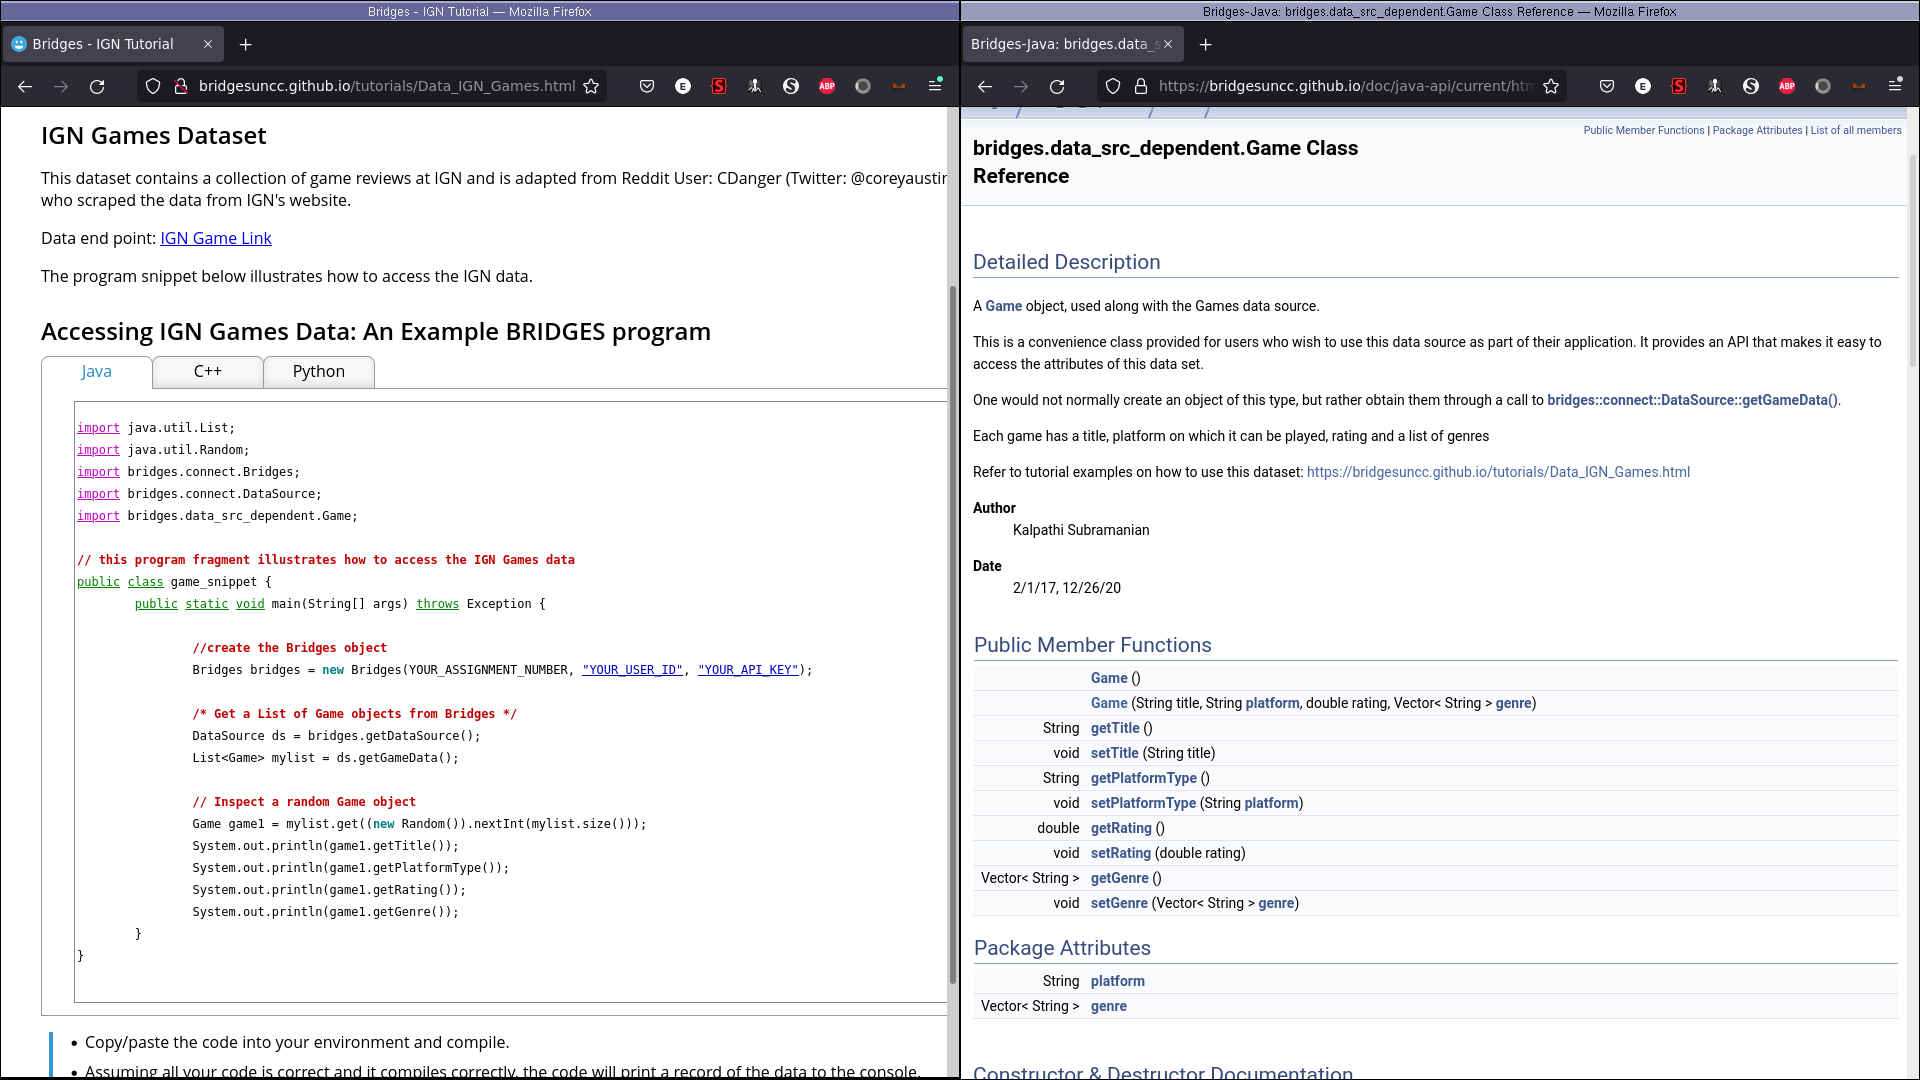
\includegraphics[width=1.02\linewidth]{dataset_figs/DatasetGame.png}
\end{frame}

\begin{frame}
  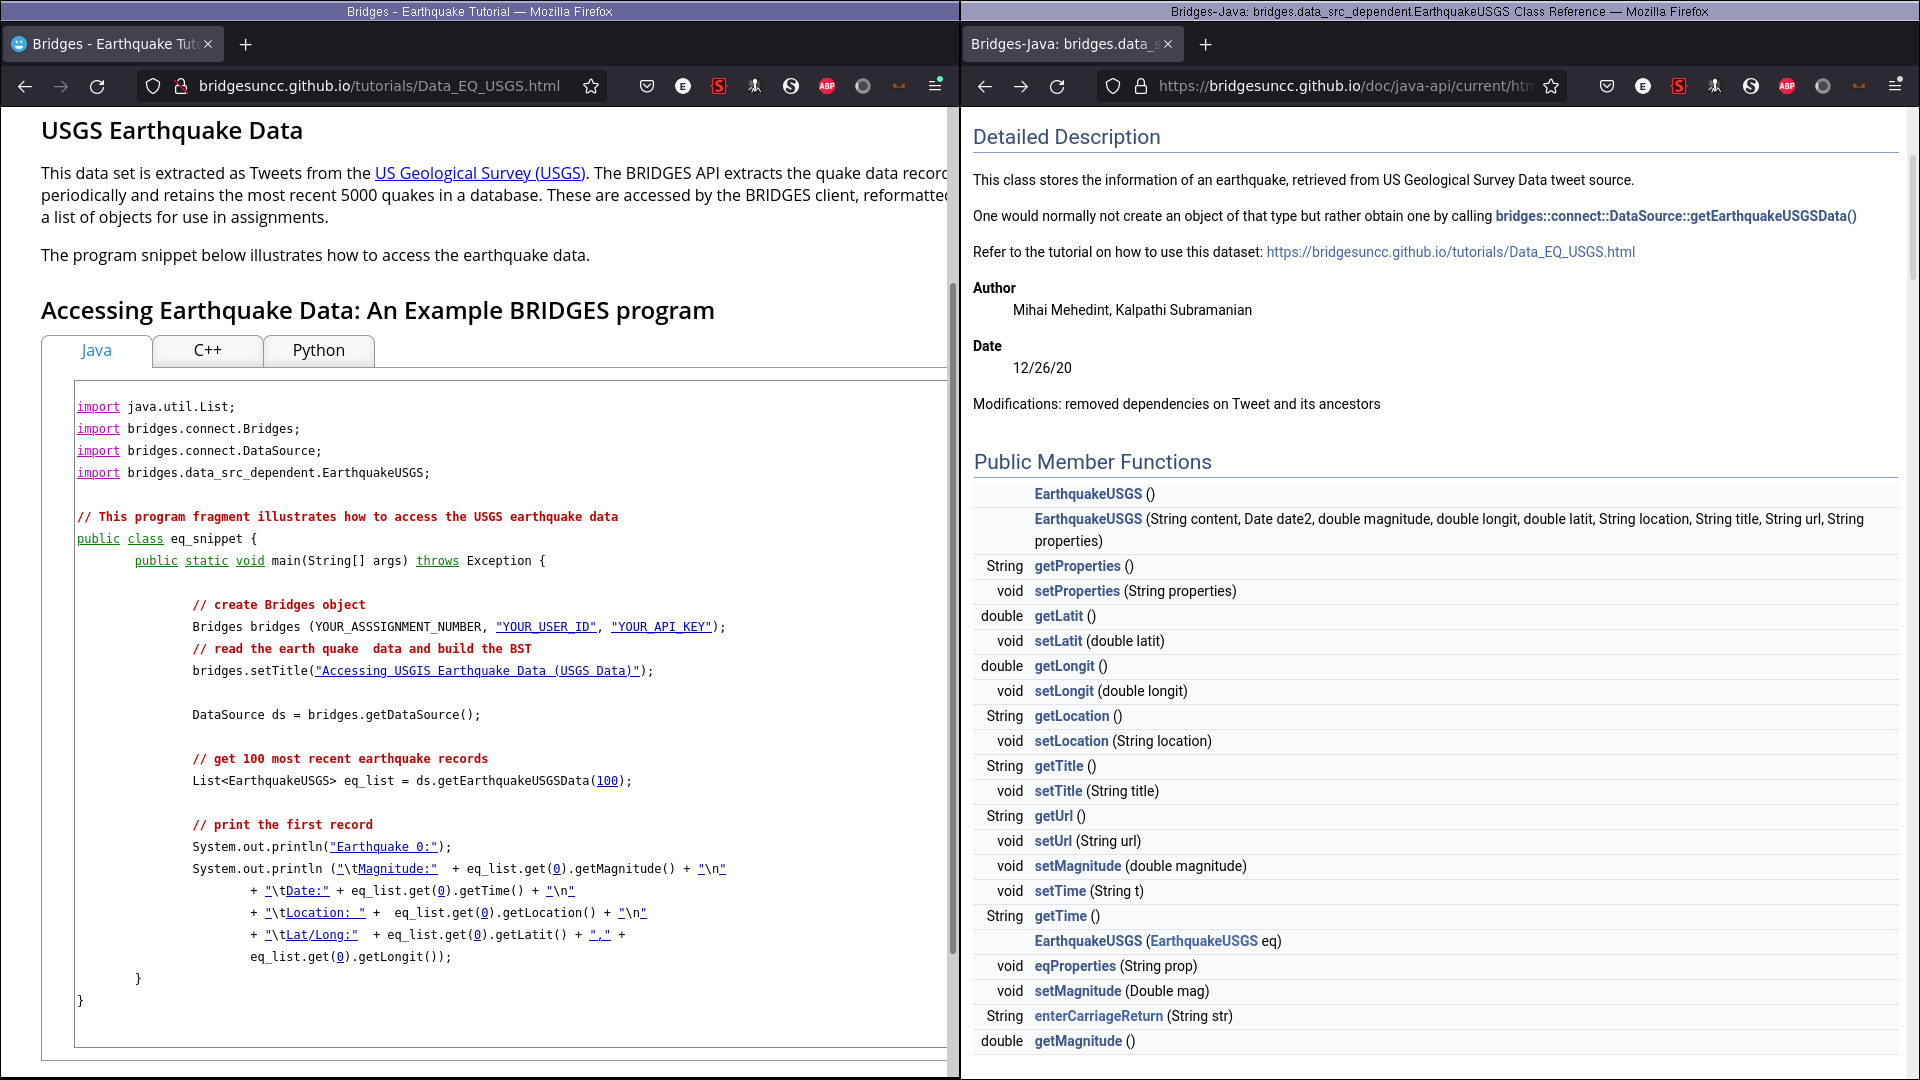
\includegraphics[width=1.02\linewidth]{dataset_figs/Earthquake.png}
\end{frame}

\begin{frame}
  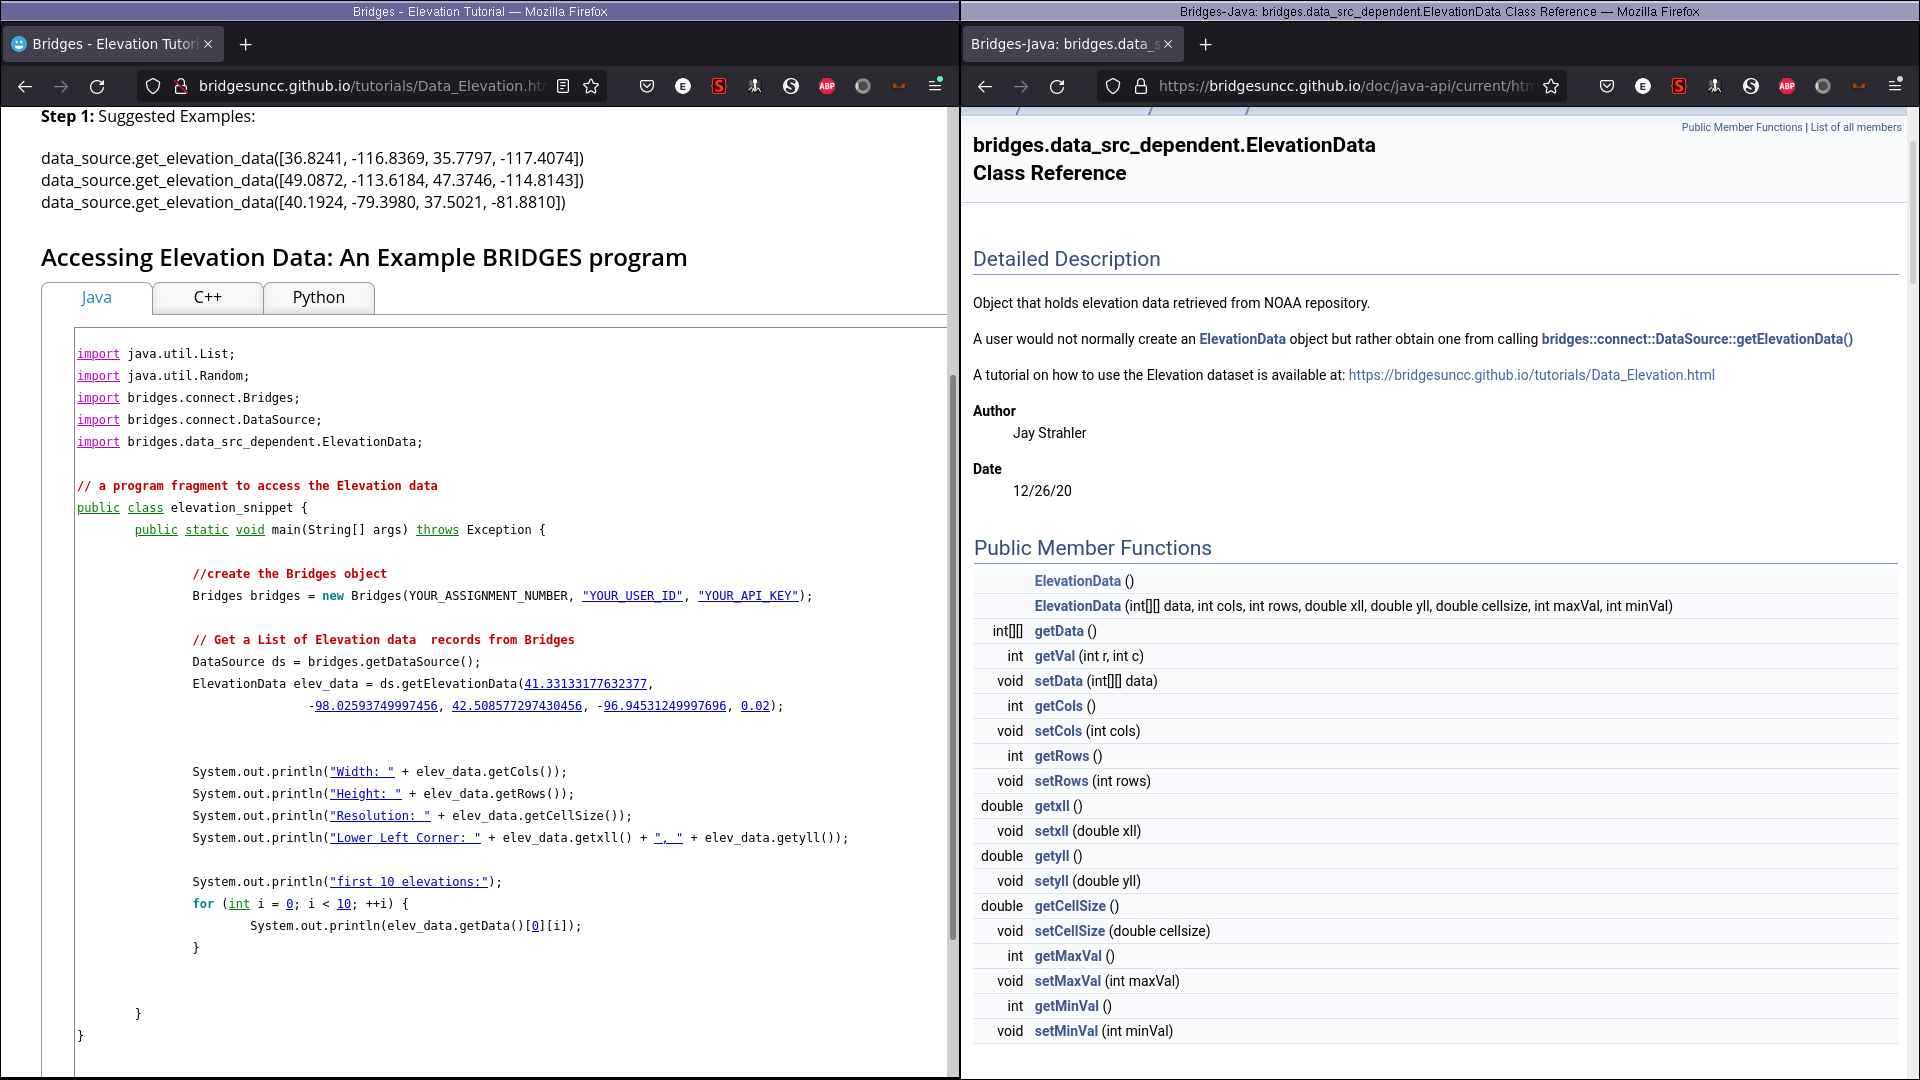
\includegraphics[width=1.02\linewidth]{dataset_figs/Elevation.png}
\end{frame}

\begin{frame}
  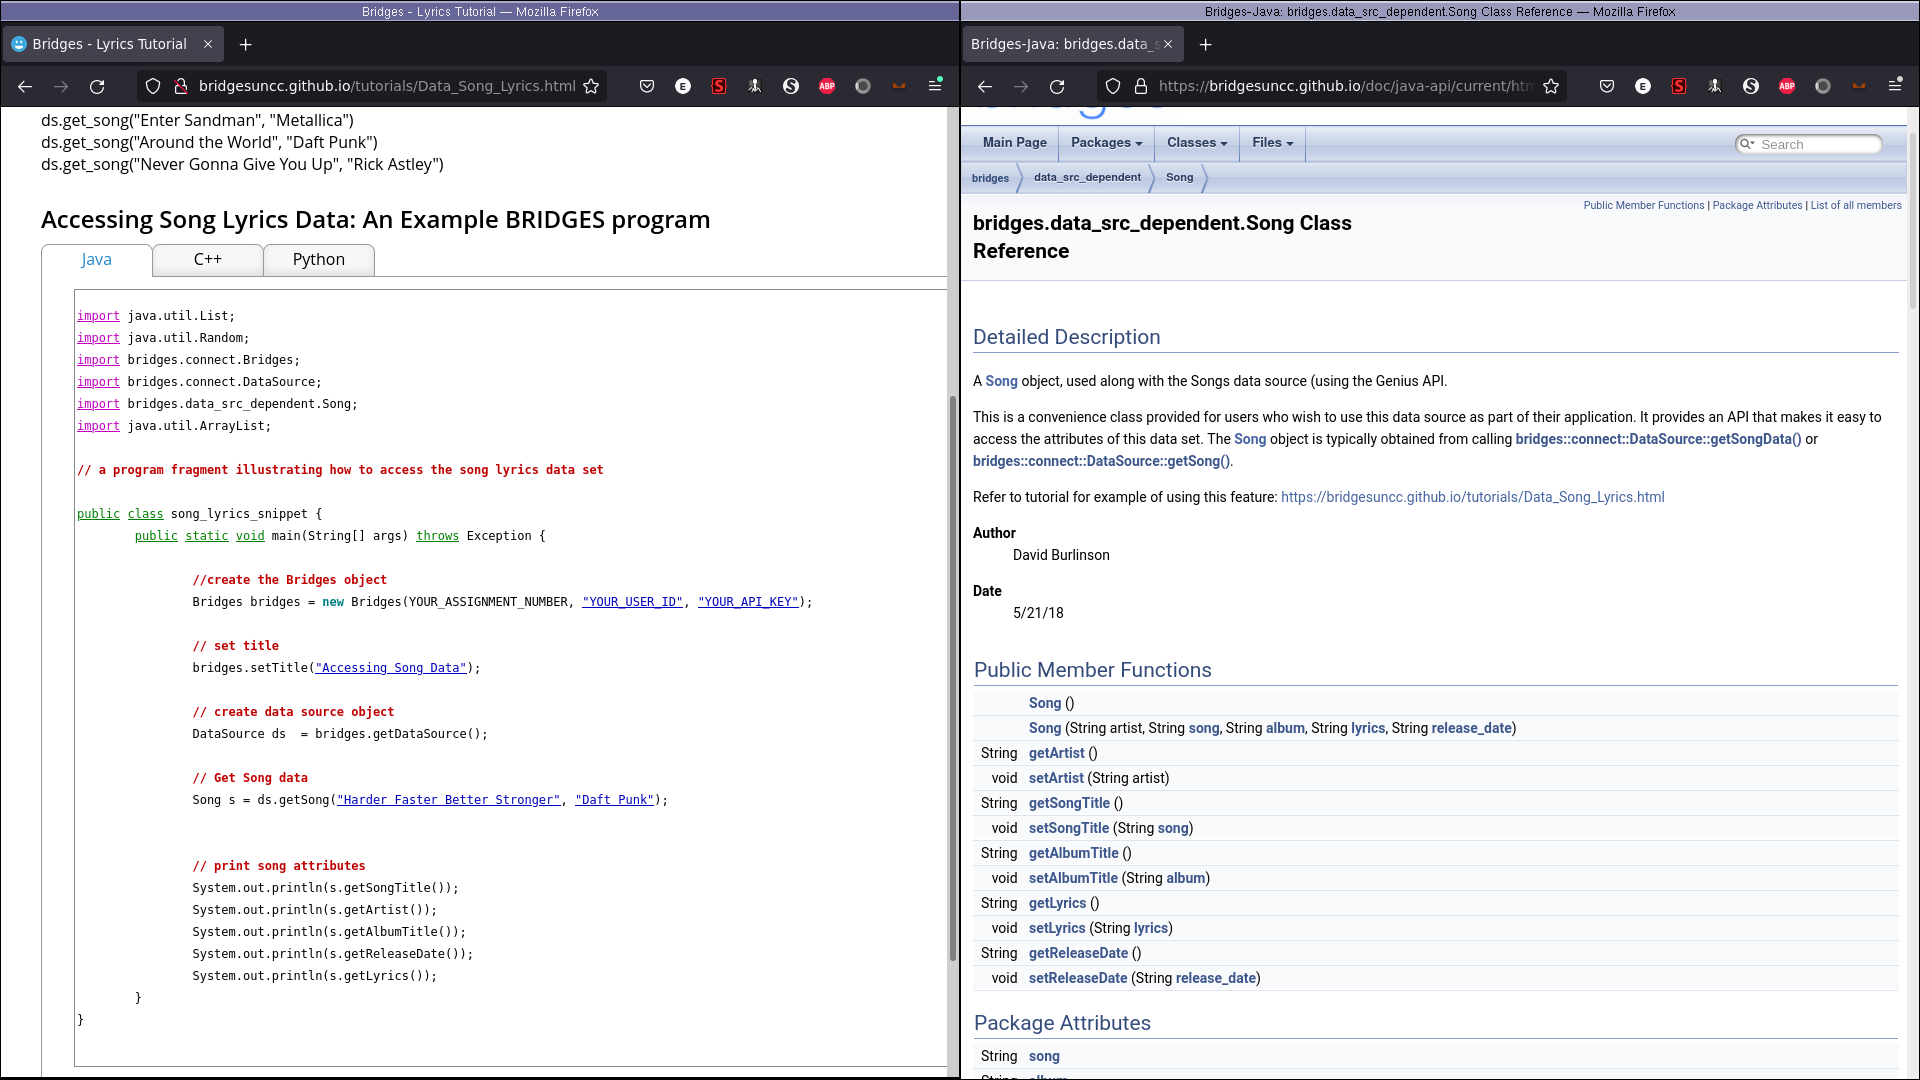
\includegraphics[width=1.02\linewidth]{dataset_figs/Song.png}
\end{frame}

\begin{frame}
  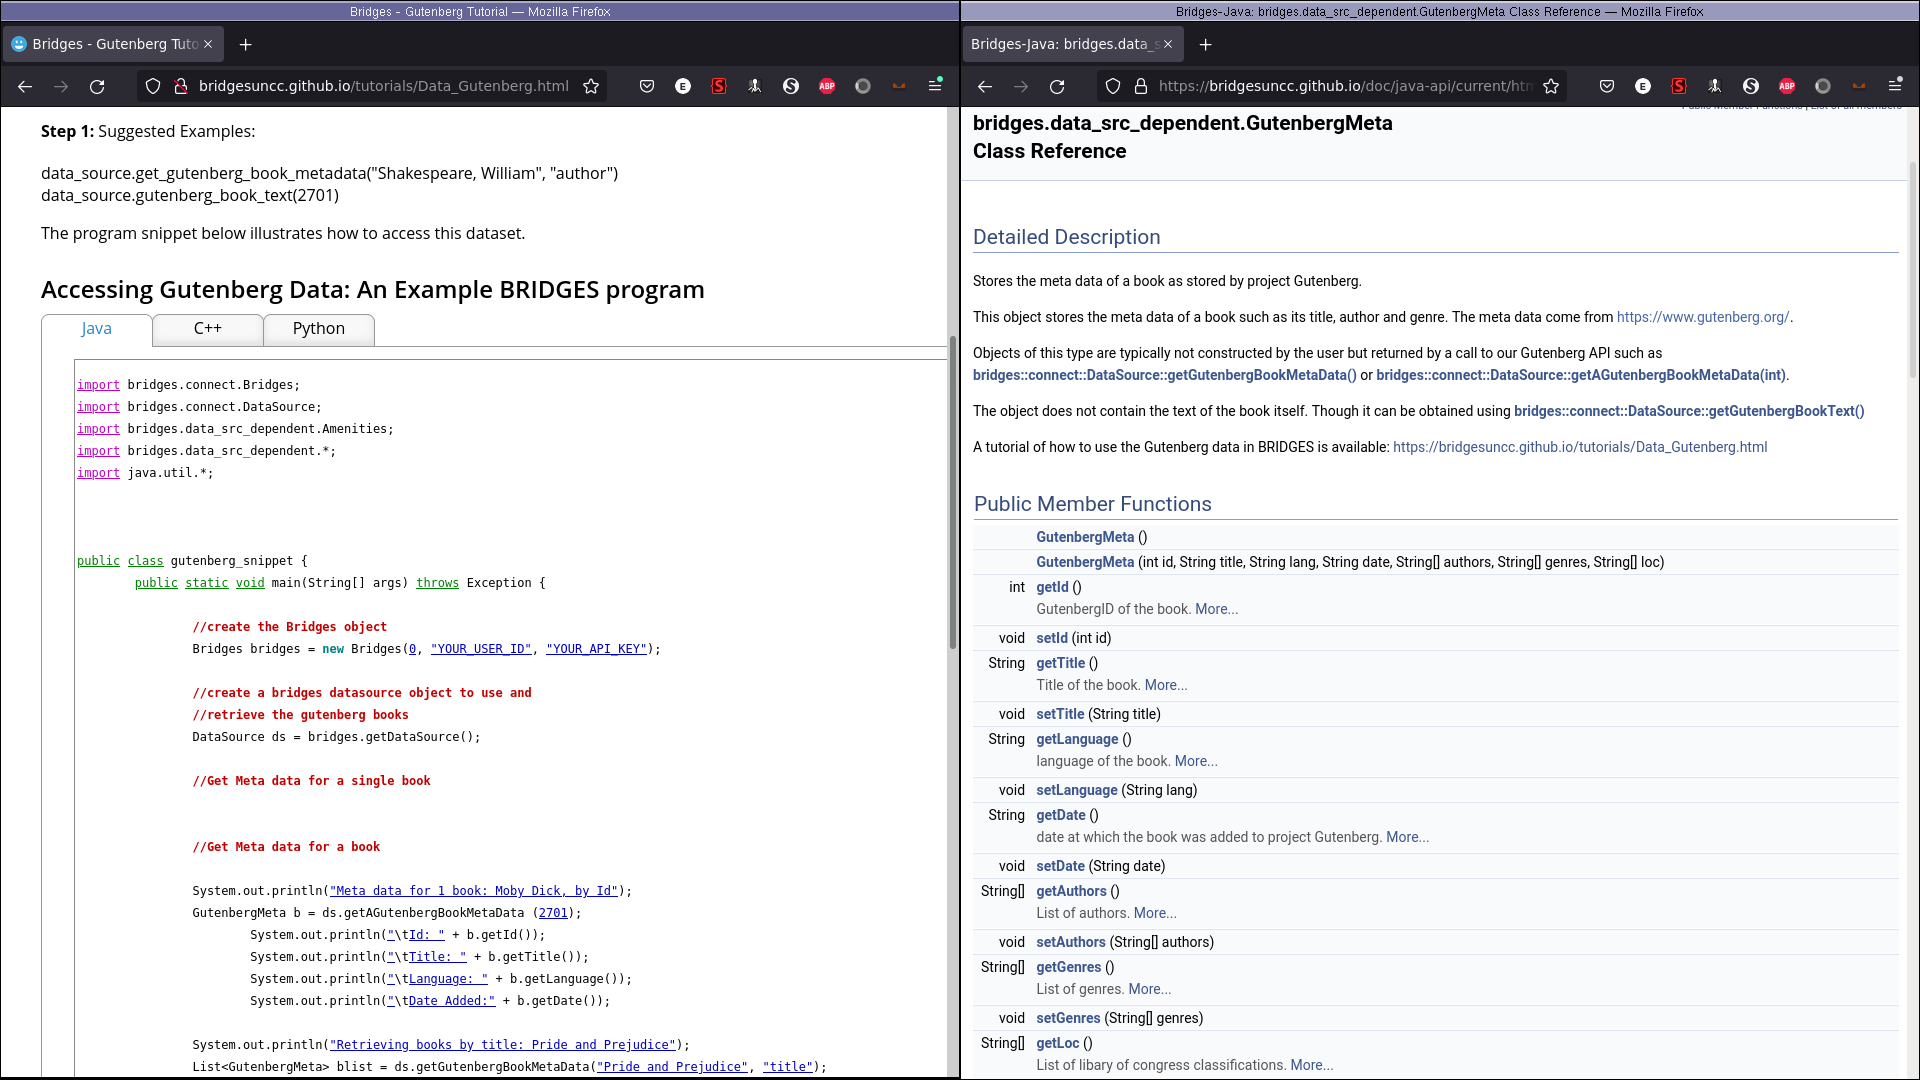
\includegraphics[width=1.02\linewidth]{dataset_figs/Gutenberg.png}
\end{frame}

\begin{frame}
  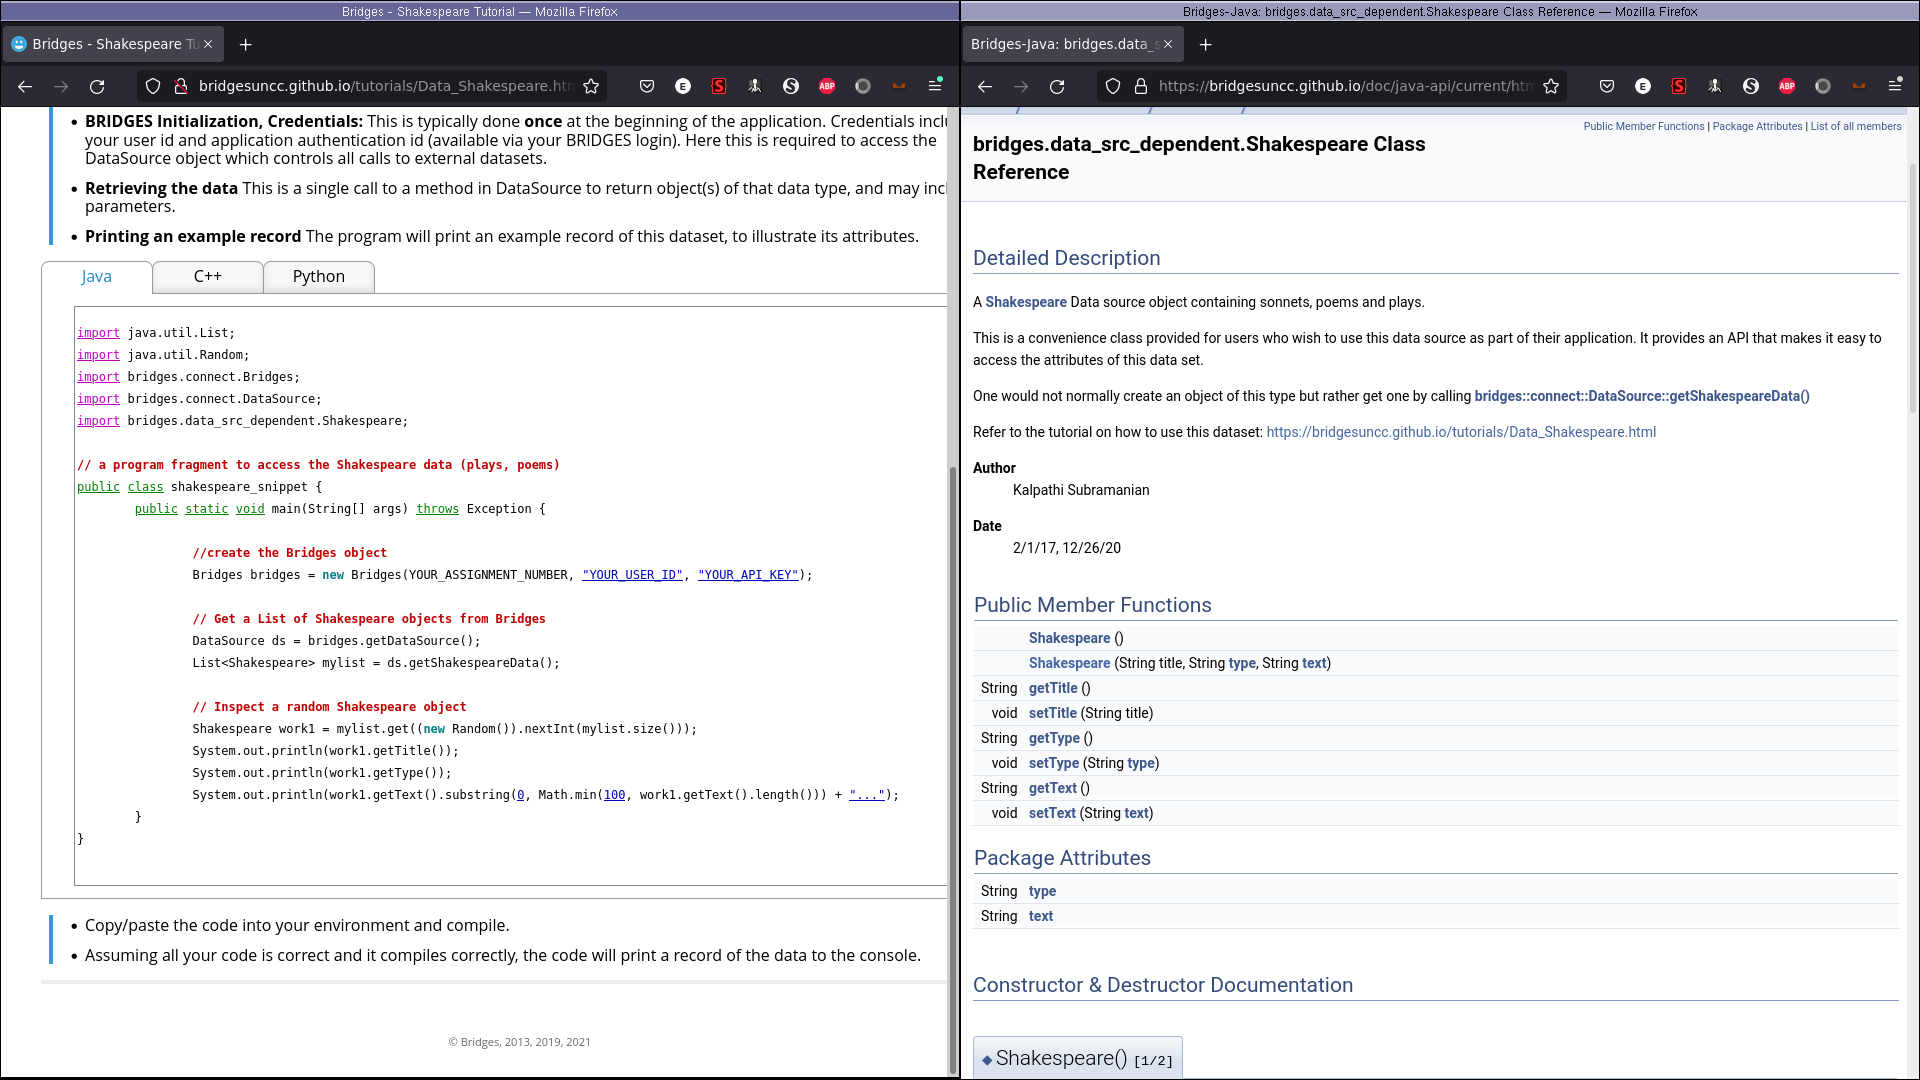
\includegraphics[width=1.02\linewidth]{dataset_figs/Shakespeare.png}
\end{frame}

\begin{frame}
  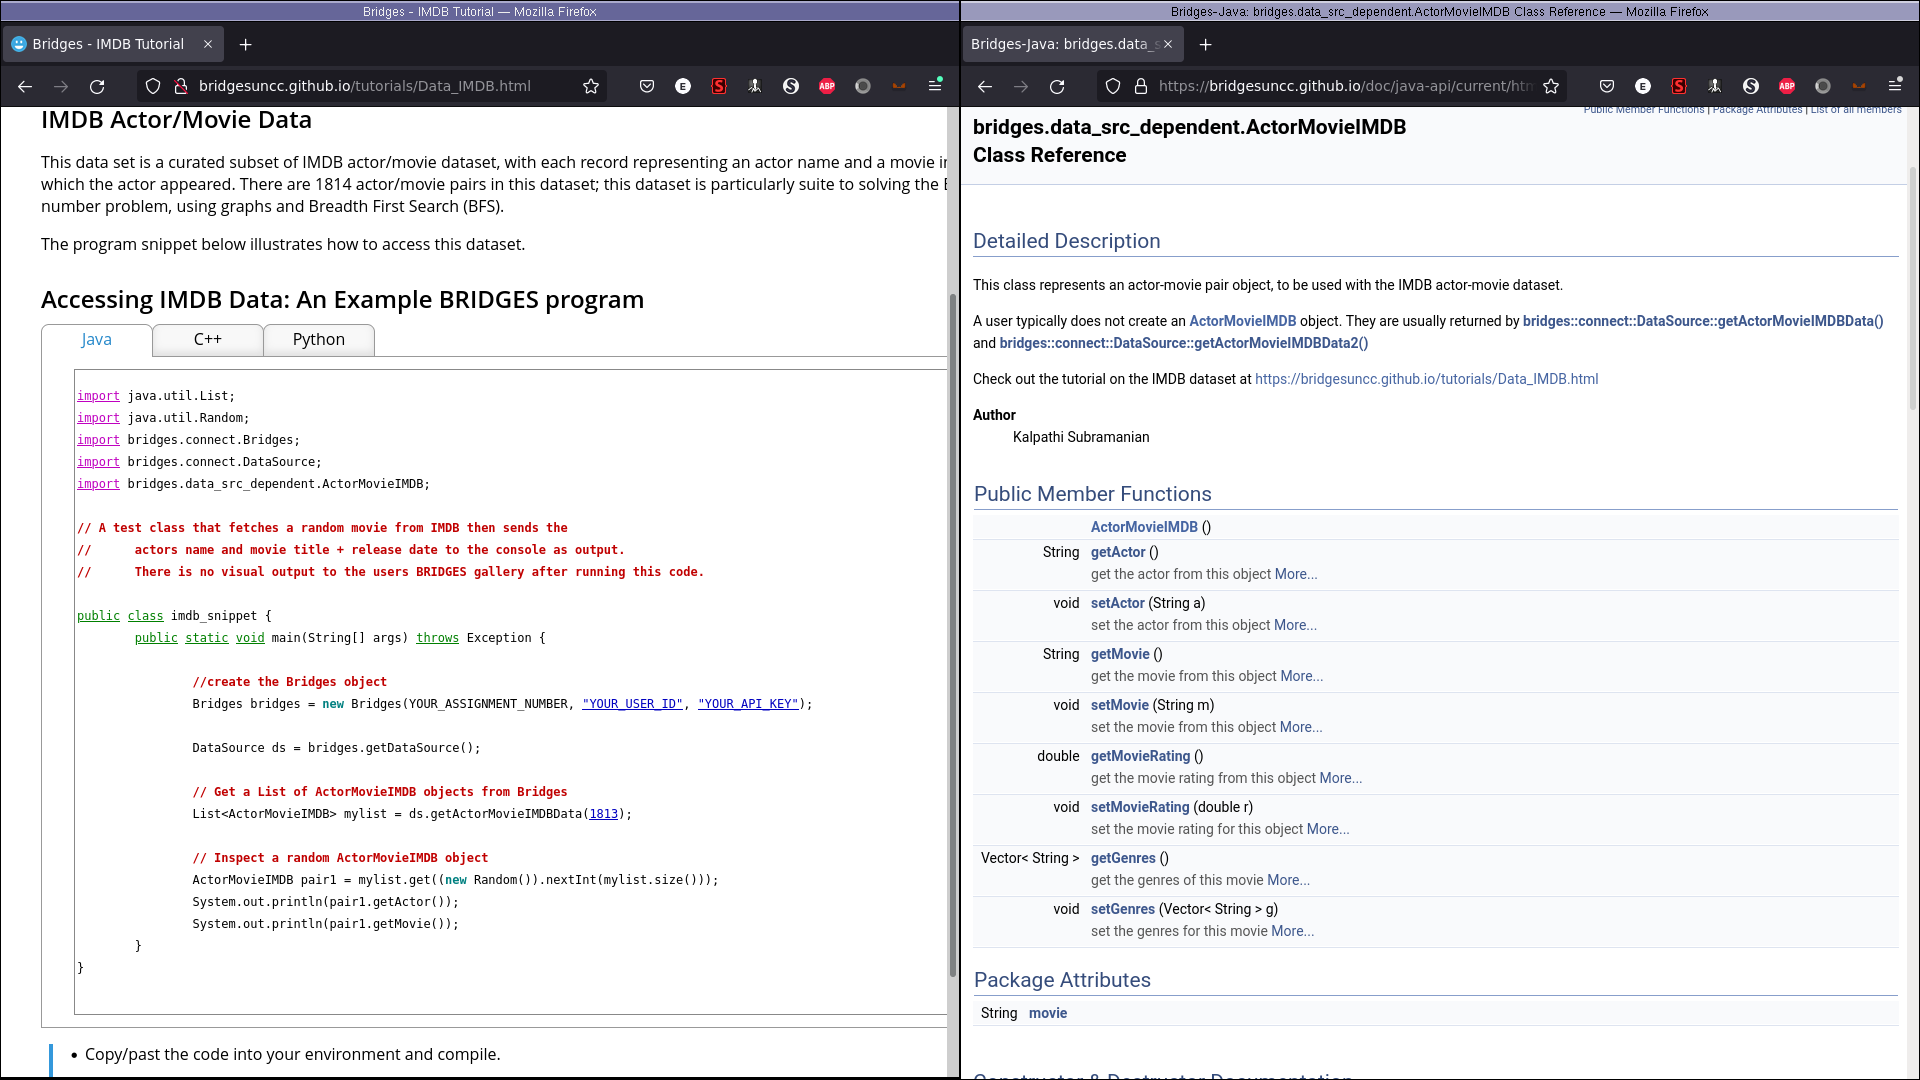
\includegraphics[width=1.02\linewidth]{dataset_figs/IMDB.png}
\end{frame}

\begin{frame}
  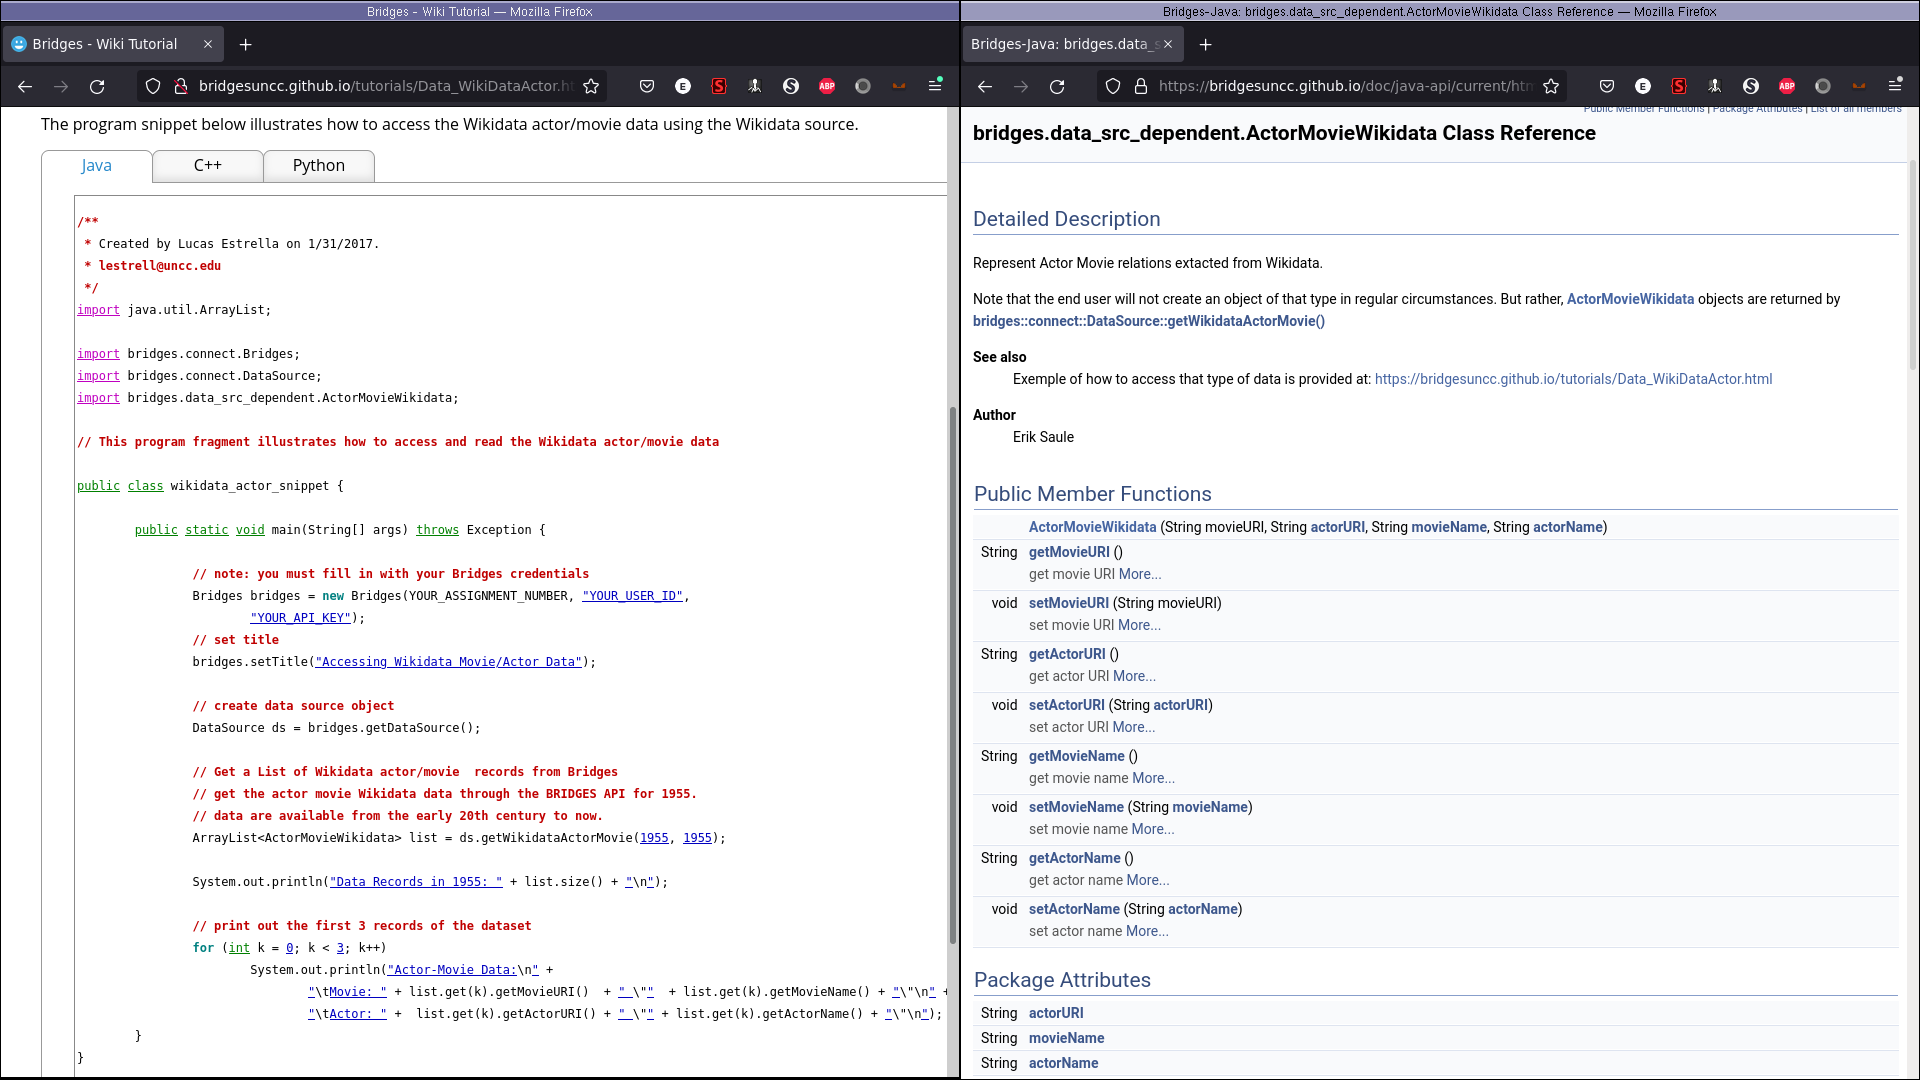
\includegraphics[width=1.02\linewidth]{dataset_figs/WikidataActor.png}
\end{frame}

\begin{frame}
  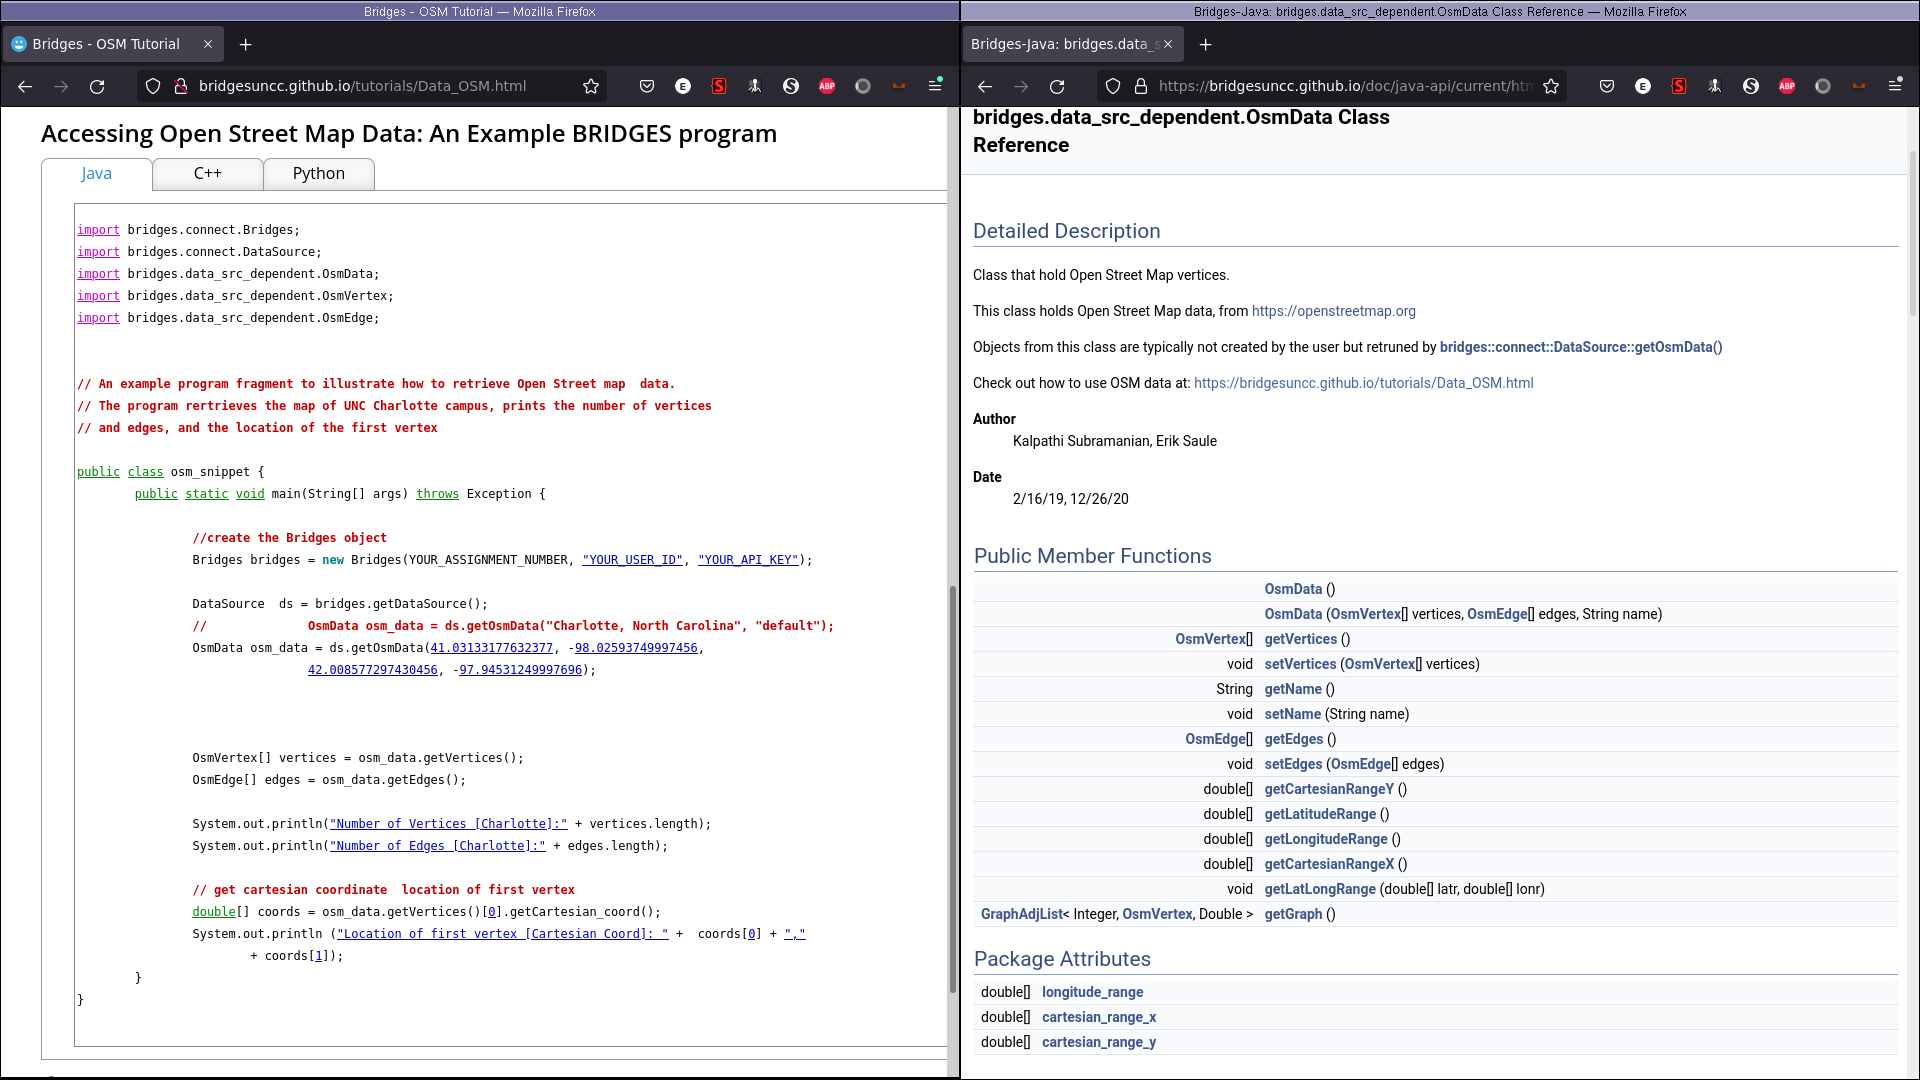
\includegraphics[width=1.02\linewidth]{dataset_figs/OSMmap.png}
\end{frame}

\begin{frame}
  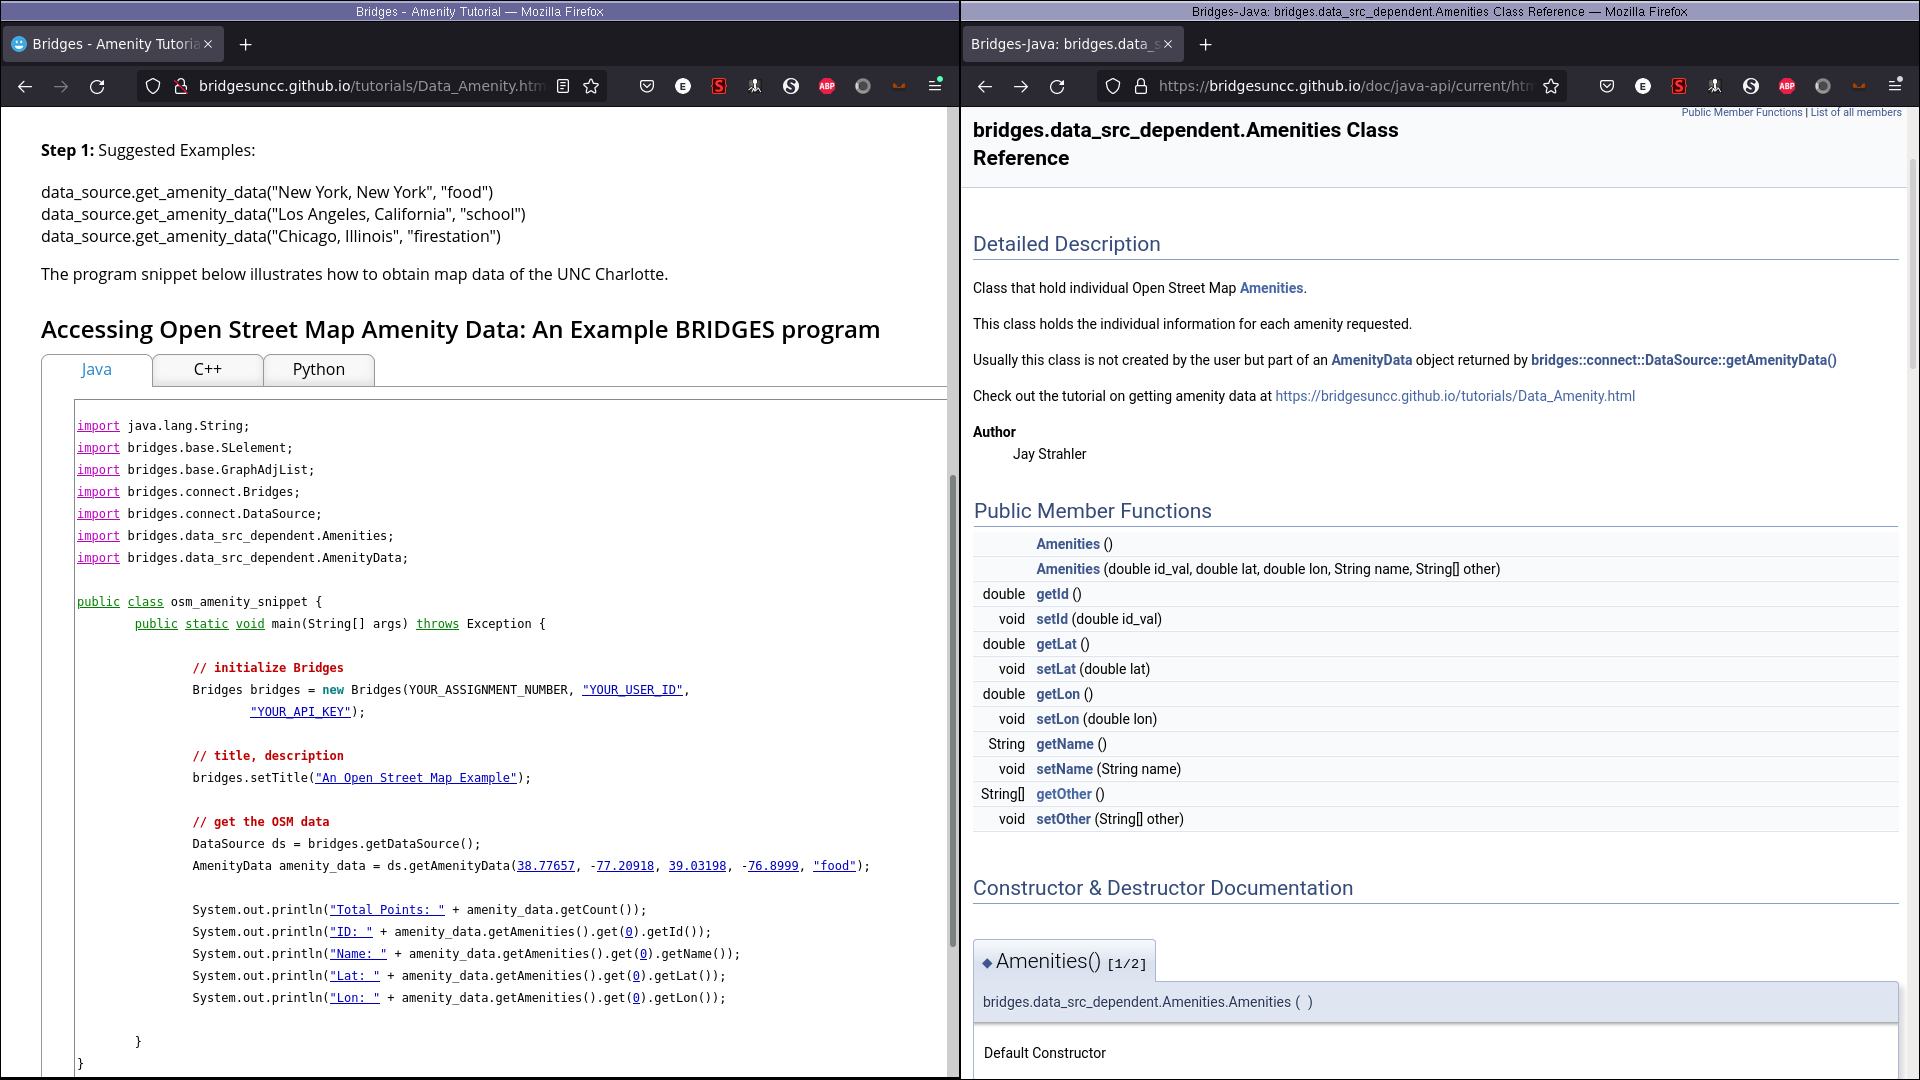
\includegraphics[width=1.02\linewidth]{dataset_figs/OSMAmenities.png}
\end{frame}

\section{Visualizations}

\begin{frame}
  \frametitle{Arrays}

  \begin{columns}
    \column{.45\linewidth}
    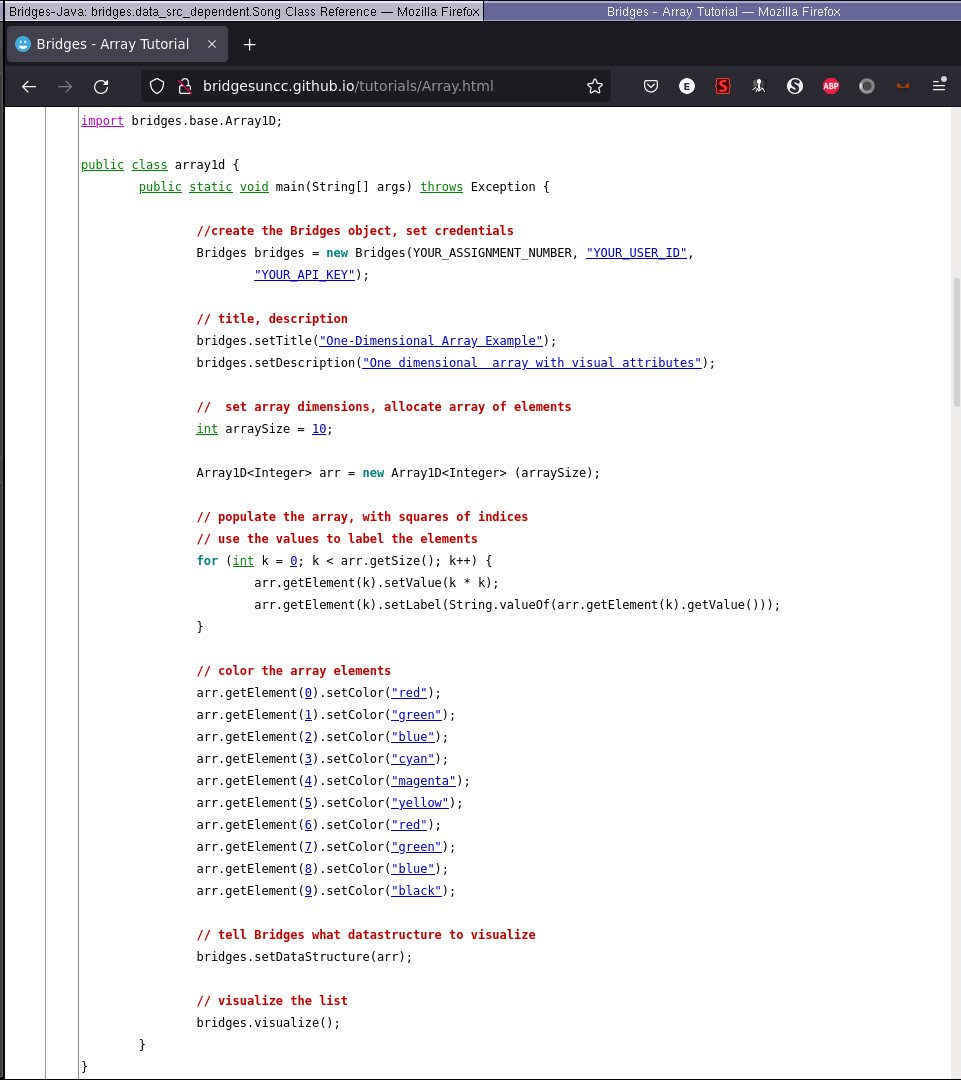
\includegraphics[width=1.0\linewidth]{viz_figs/ArrayCode.png}
    
    \column{.45\linewidth}

    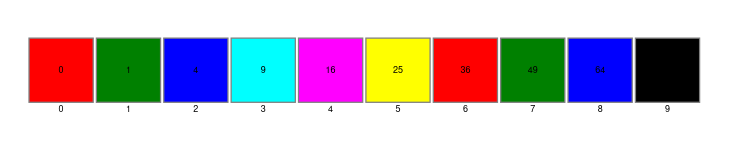
\includegraphics[width=1.0\linewidth]{viz_figs/Array1Dout.png}

    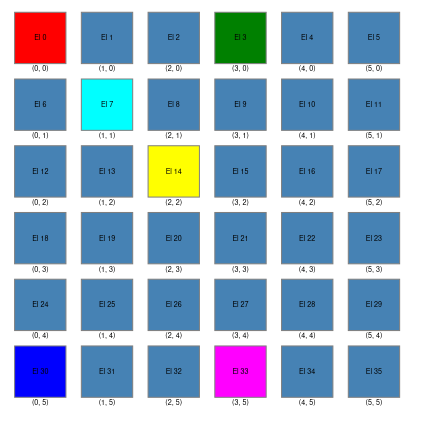
\includegraphics[width=.5\linewidth]{viz_figs/Array2Dout.png}

    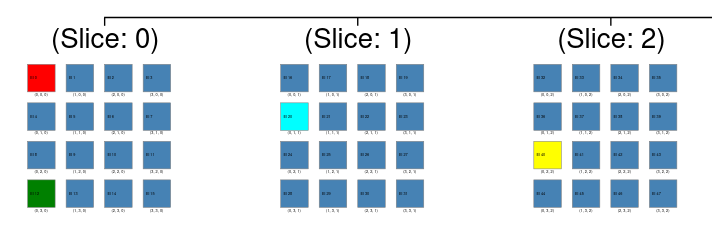
\includegraphics[width=1.0\linewidth]{viz_figs/Array3Dout.png}
  \end{columns}
\end{frame}


\begin{frame}
  \frametitle{AudioClip}

  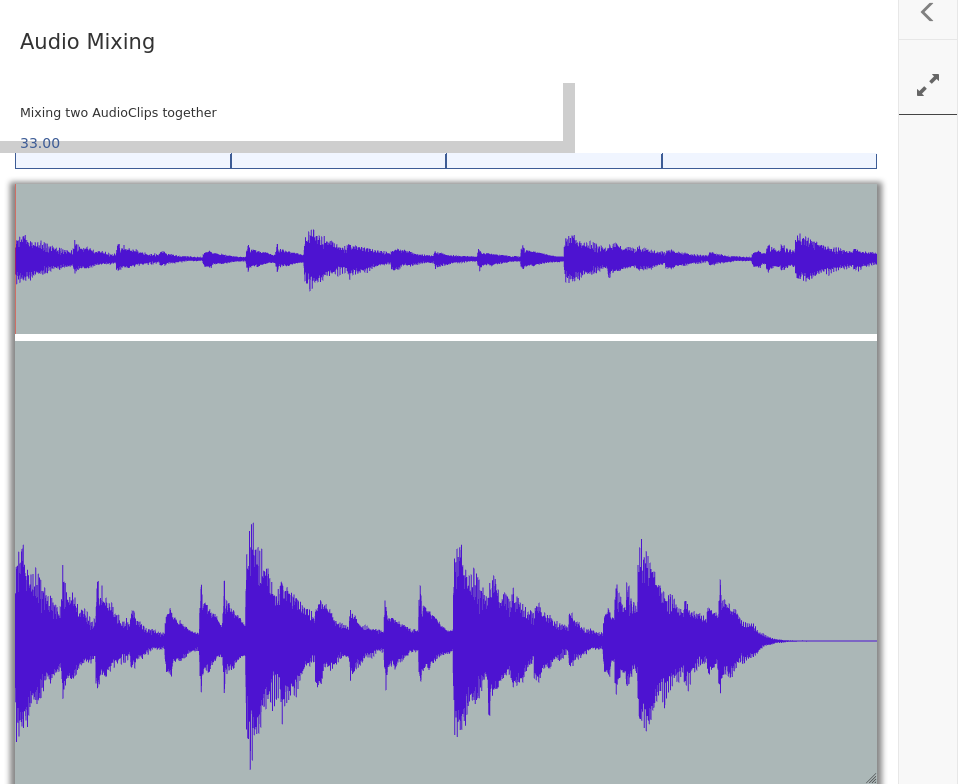
\includegraphics[width=.7\linewidth]{viz_figs/AudioClip1.png}
\end{frame}


\begin{frame}
  \frametitle{LineChart}
  
  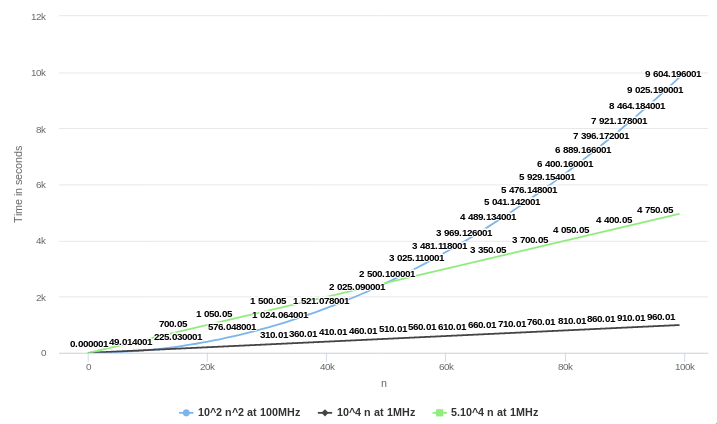
\includegraphics[width=.7\linewidth]{viz_figs/LineChart.png}
\end{frame}

\begin{frame}
  \frametitle{ColorGrid}

  \begin{columns}
    \column{.3\linewidth}
    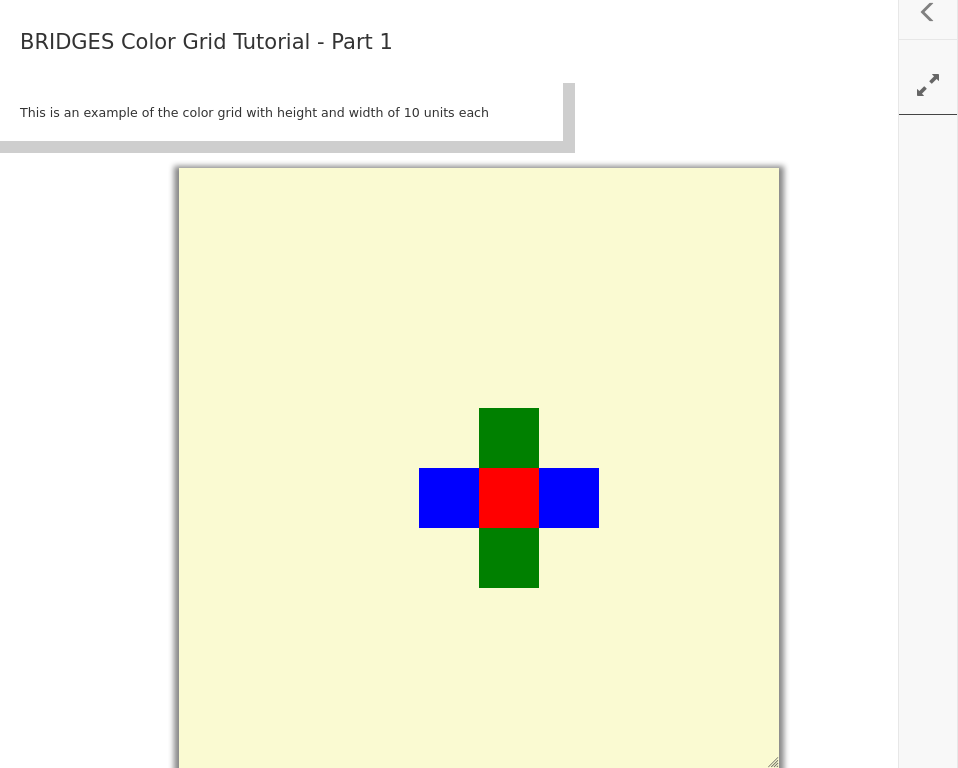
\includegraphics[width=1.0\linewidth]{viz_figs/ColorGrid1.png}
    
    \column{.3\linewidth}
    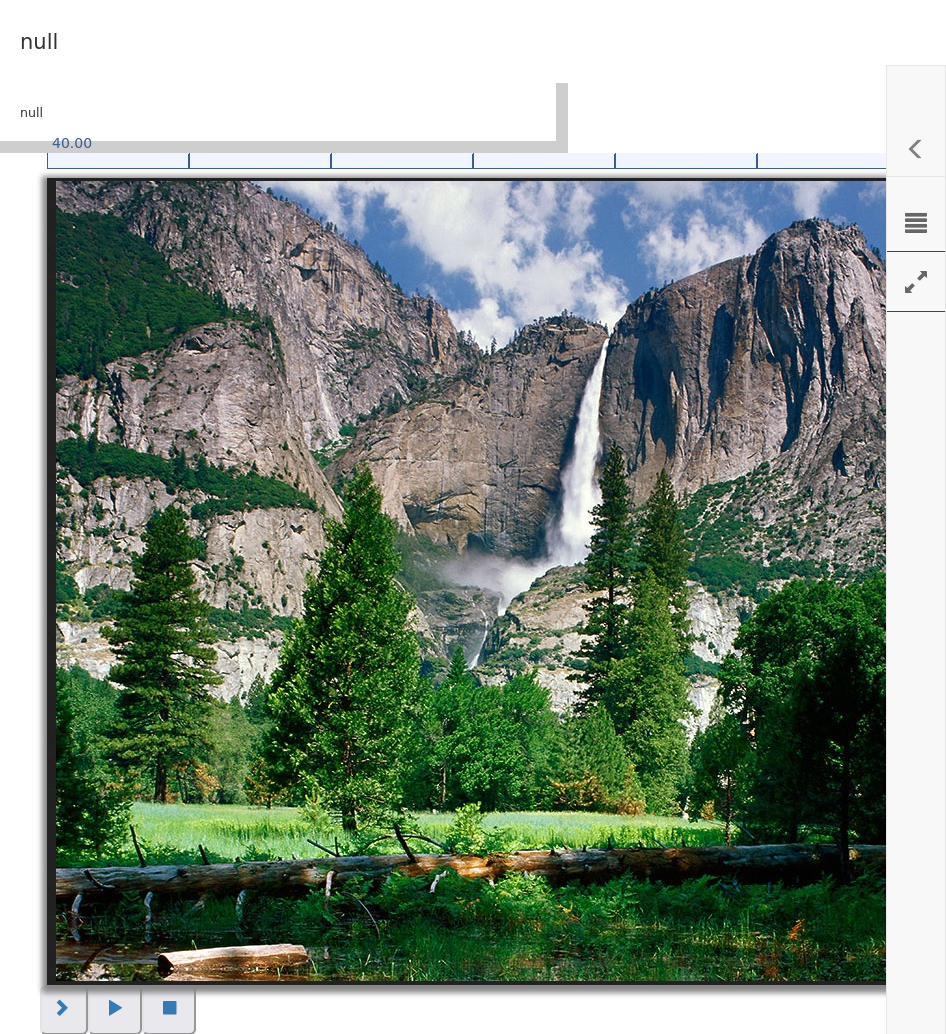
\includegraphics[width=1.0\linewidth]{viz_figs/ColorGrid2.png}

    \column{.3\linewidth}
    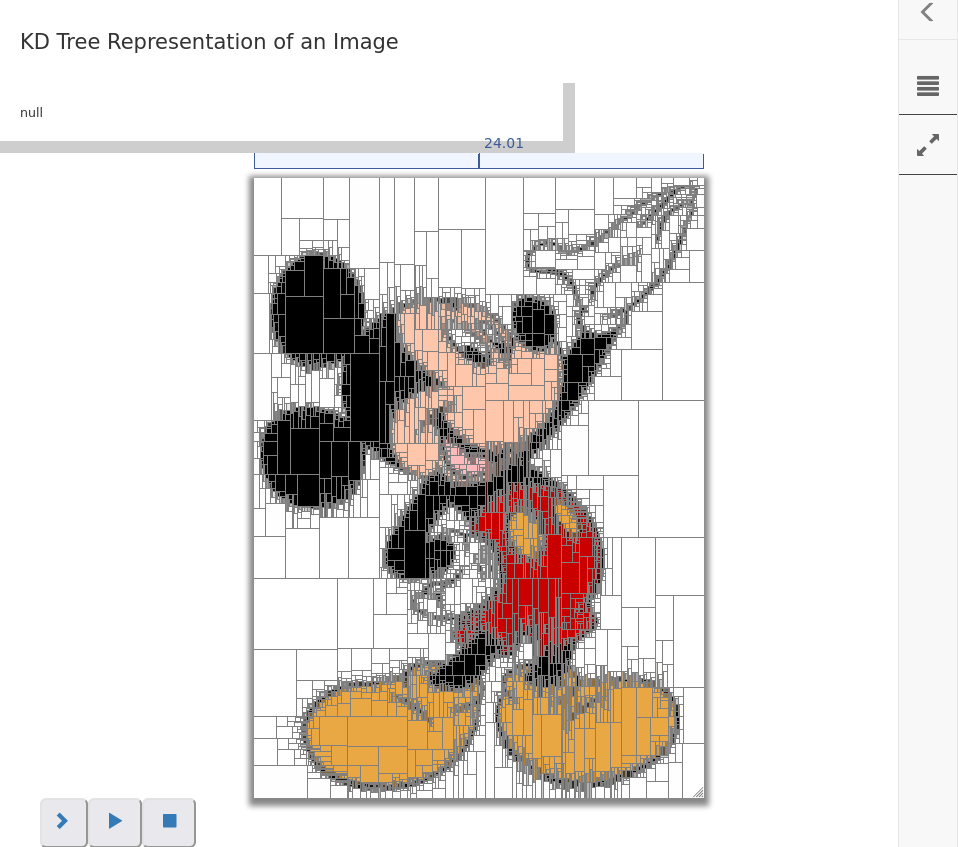
\includegraphics[width=1.\linewidth]{viz_figs/ColorGrid3.png}
  \end{columns}
\end{frame}

\begin{frame}
  \frametitle{Games}

  \begin{columns}
    \column{.3\linewidth}
    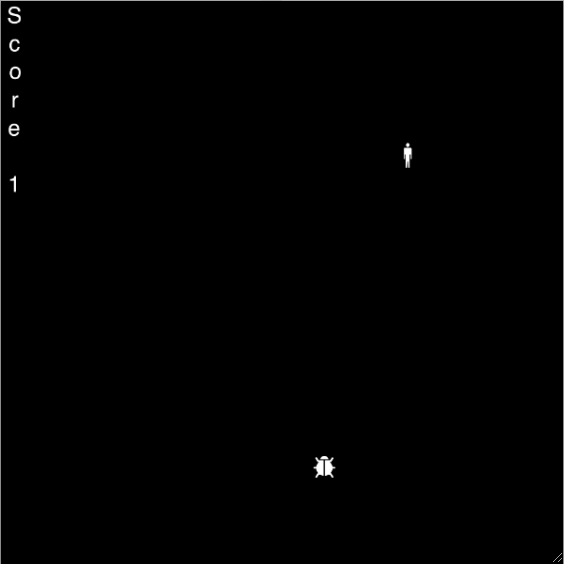
\includegraphics[width=1.0\linewidth]{viz_figs/game-bugstomp.png}

    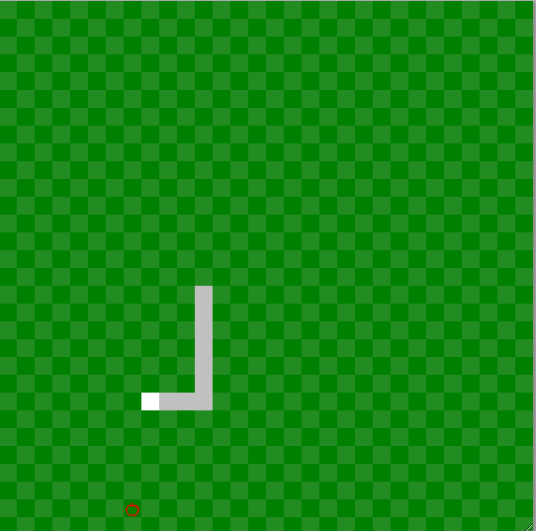
\includegraphics[width=1.0\linewidth]{viz_figs/game-snake.png}
    
    \column{.3\linewidth}
    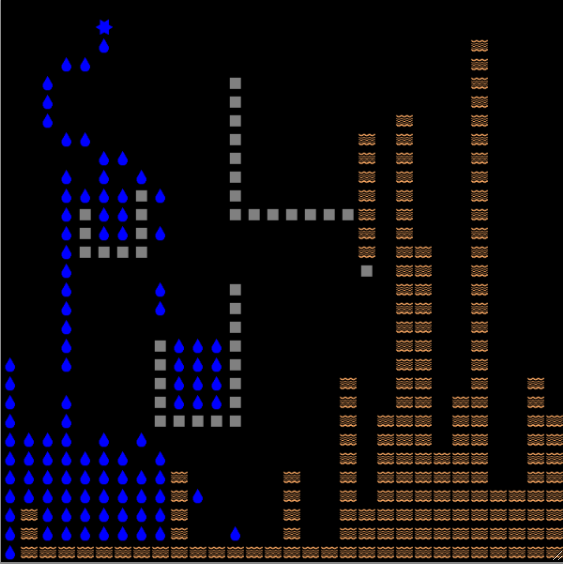
\includegraphics[width=1.0\linewidth]{viz_figs/game-fallingsand.png}

    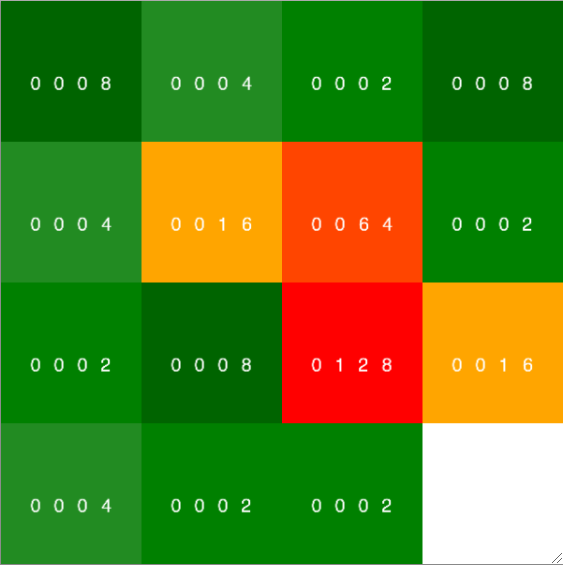
\includegraphics[width=1.0\linewidth]{viz_figs/game-2048.png}
  \end{columns}
  
\end{frame}


\begin{frame}
  \frametitle{Linked List}

  \begin{columns}
    \column{.45\linewidth}
    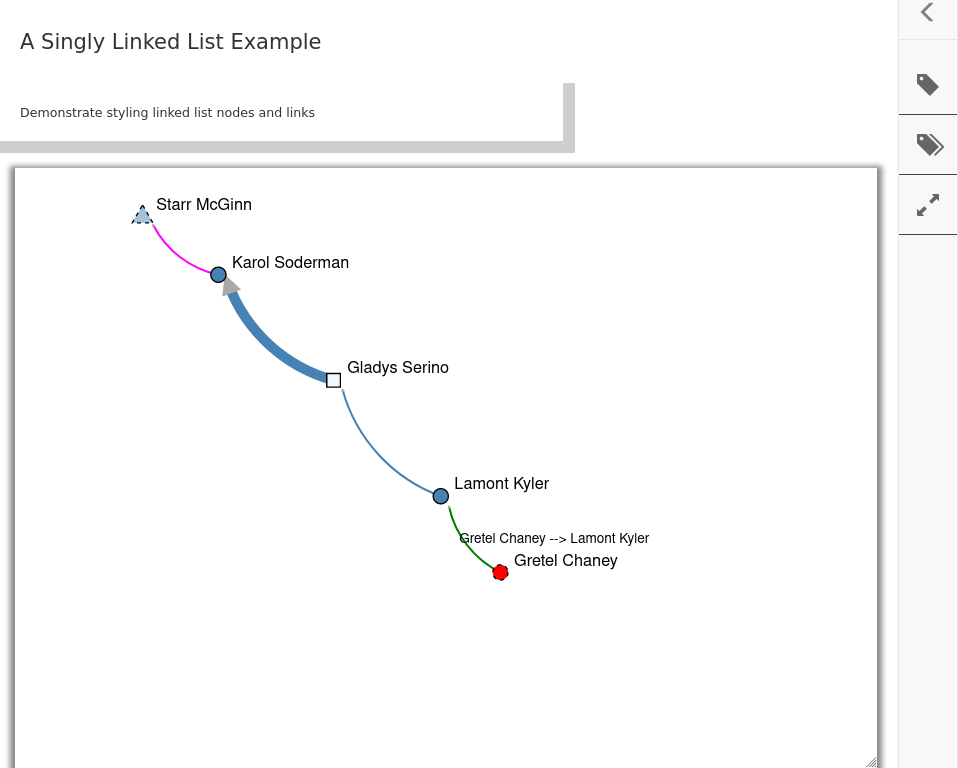
\includegraphics[width=1\linewidth]{viz_figs/LinkedList1.png}

    \column{.45\linewidth}
    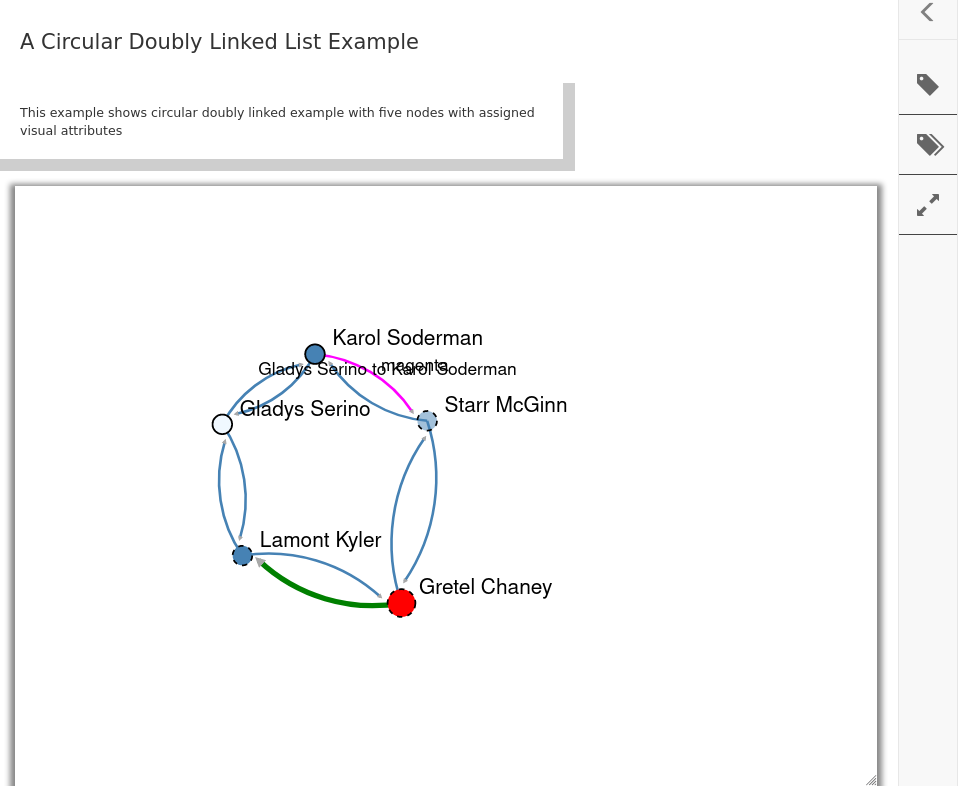
\includegraphics[width=1\linewidth]{viz_figs/CircularList.png}
  \end{columns}
  
\end{frame}

\begin{frame}
  \frametitle{Trees}

  \begin{columns}
    \column{.45\linewidth}
    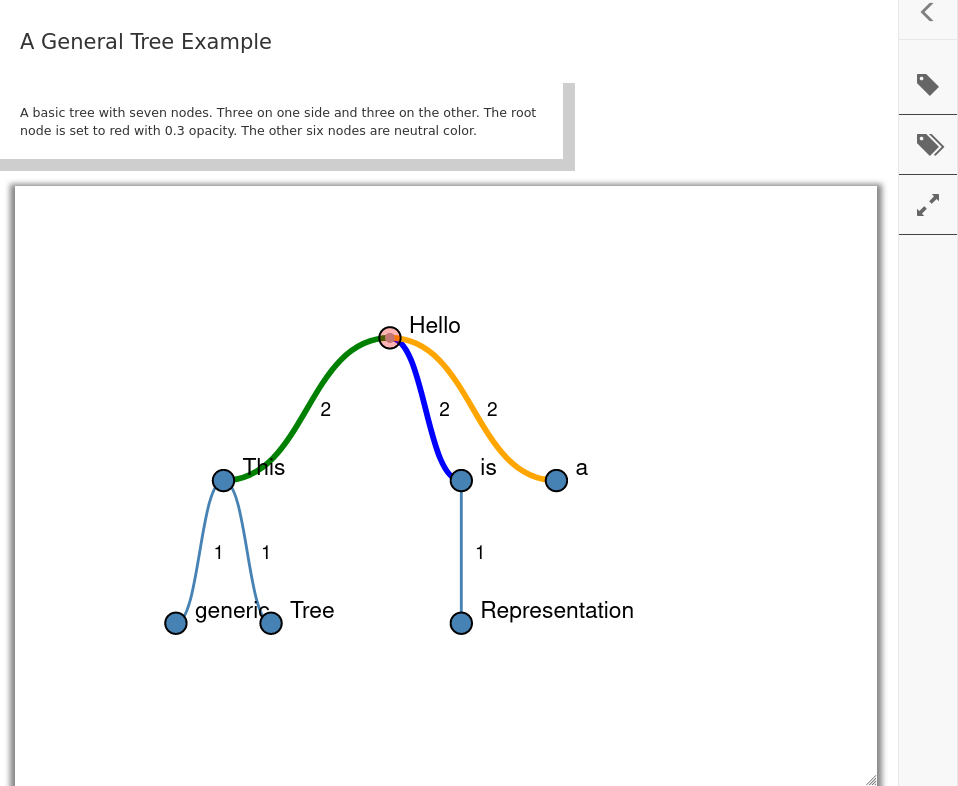
\includegraphics[width=1\linewidth]{viz_figs/Tree1.png}

    \column{.45\linewidth}
    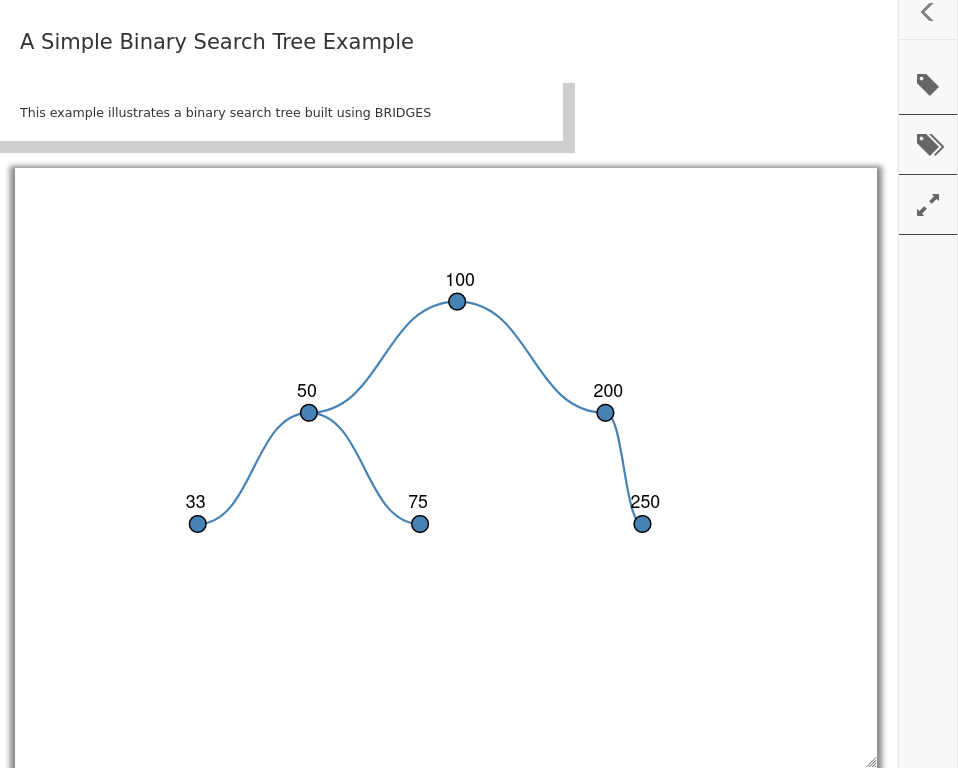
\includegraphics[width=1\linewidth]{viz_figs/Tree2.png}
  \end{columns}  
\end{frame}

\begin{frame}
  \frametitle{Graphs}
  \begin{columns}
    \column{.45\linewidth}
    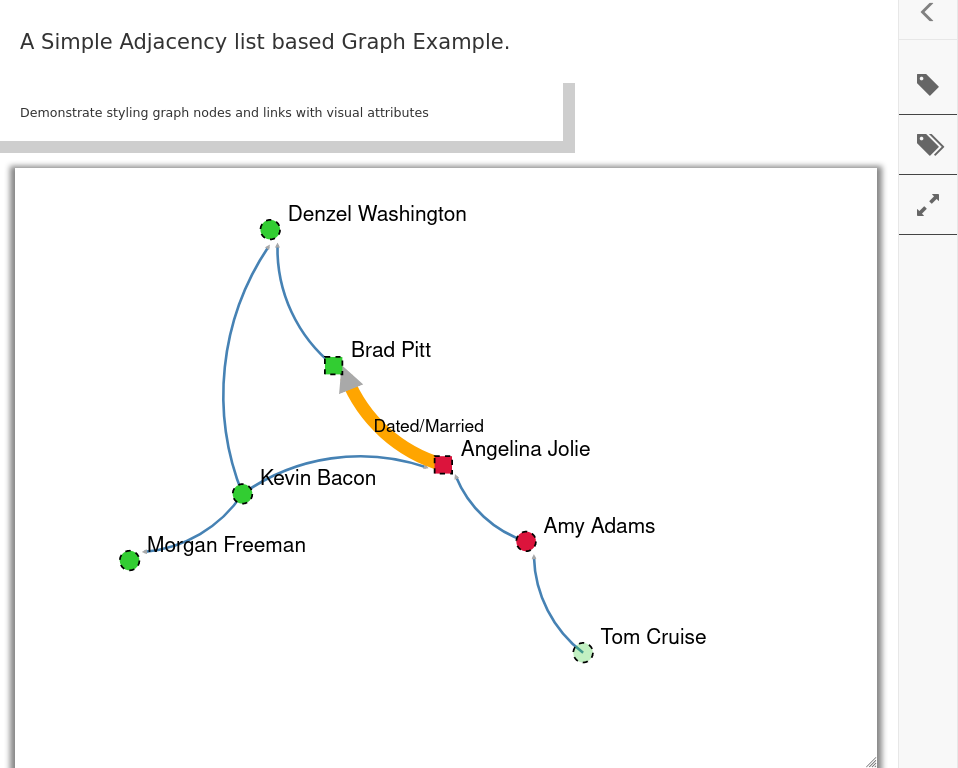
\includegraphics[width=1\linewidth]{viz_figs/Graph1.png}

    \column{.45\linewidth}
    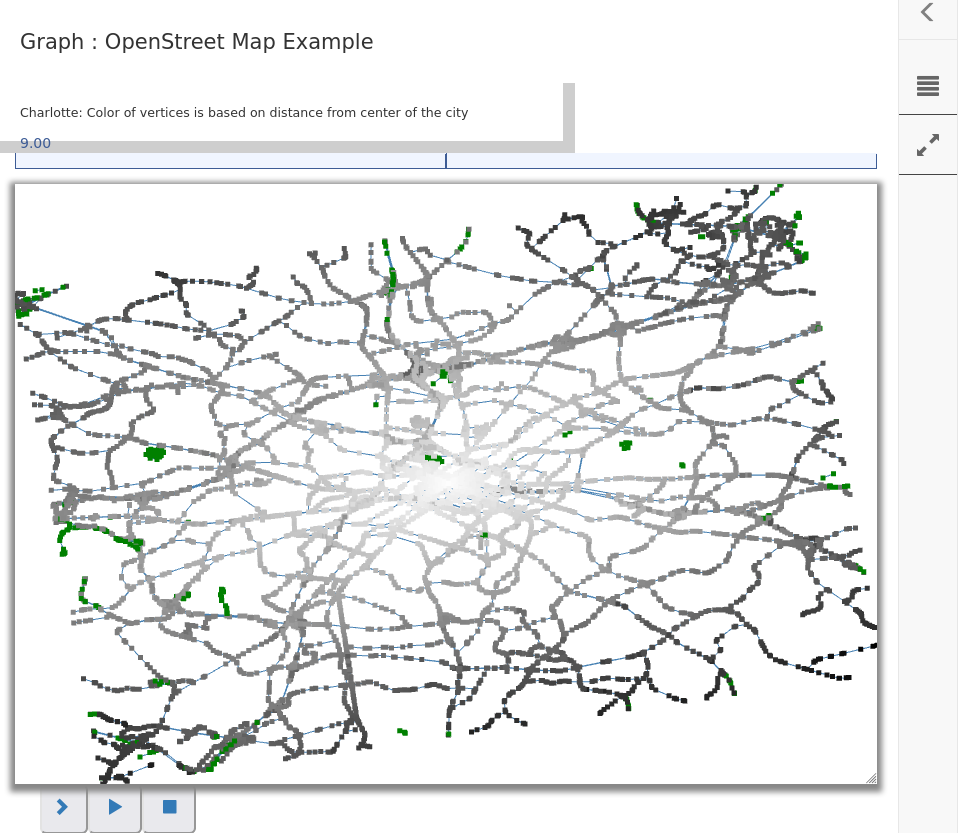
\includegraphics[width=1\linewidth]{viz_figs/Graph2.png}
  \end{columns}  
\end{frame}


\begin{frame}
  \frametitle{Shape Collection}

  \begin{columns}
    \column{.4\linewidth}
    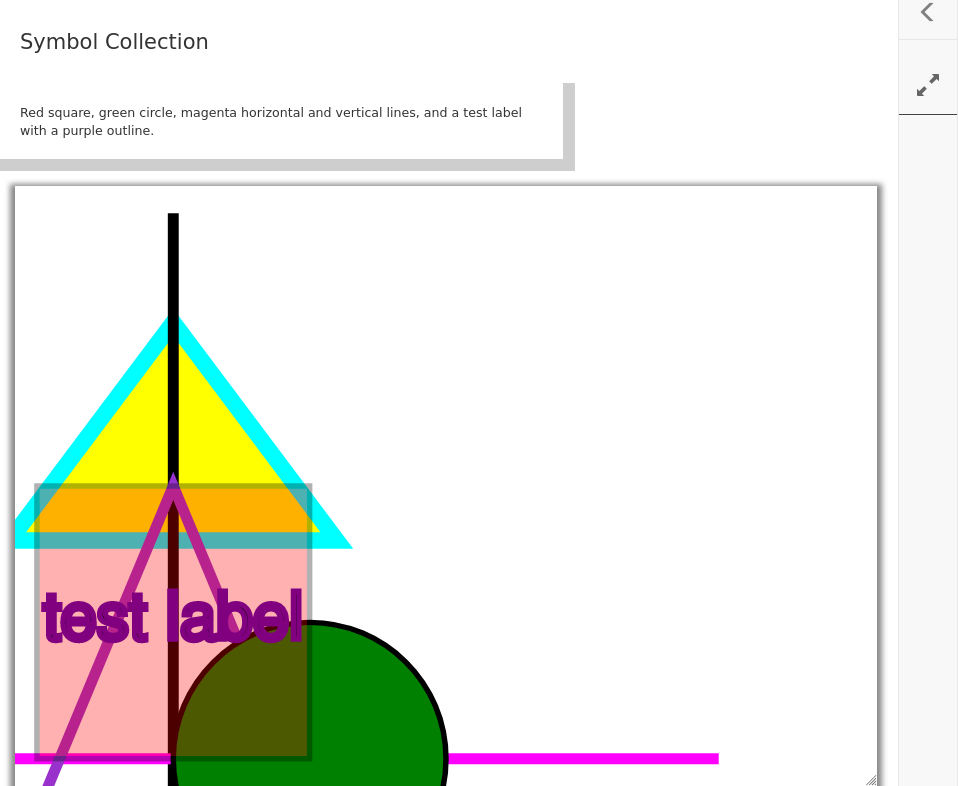
\includegraphics[width=1\linewidth]{viz_figs/Shape1.png}

    \column{.4\linewidth}
    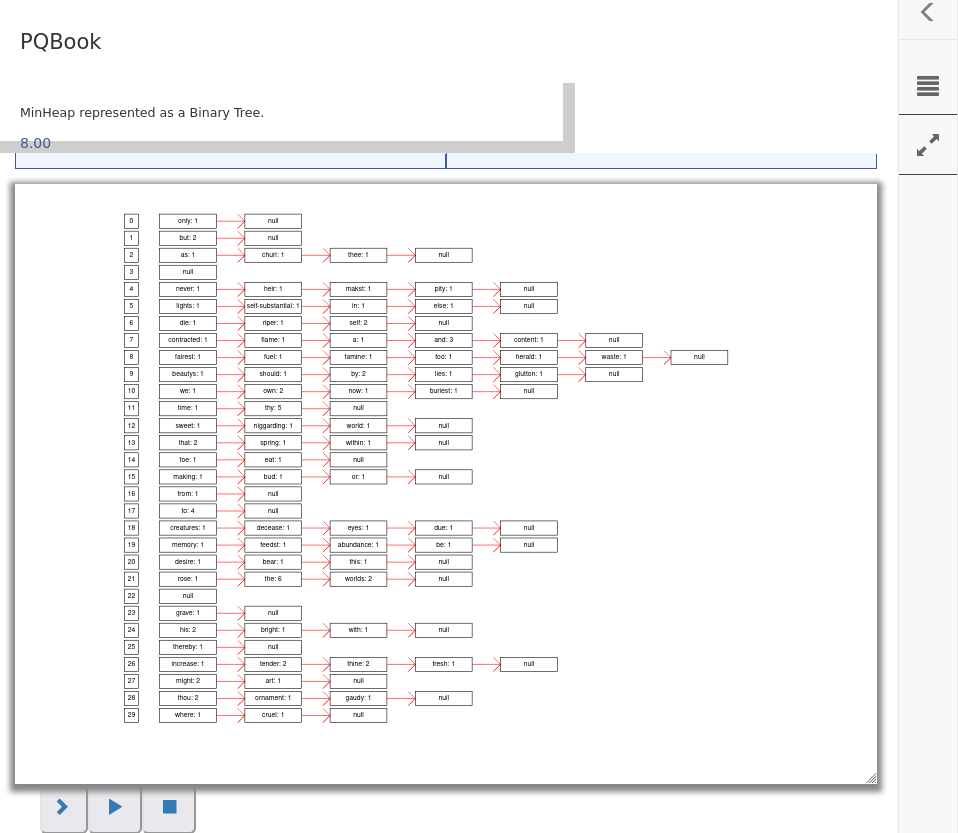
\includegraphics[width=1\linewidth]{viz_figs/Shape2.png}
  \end{columns}  

  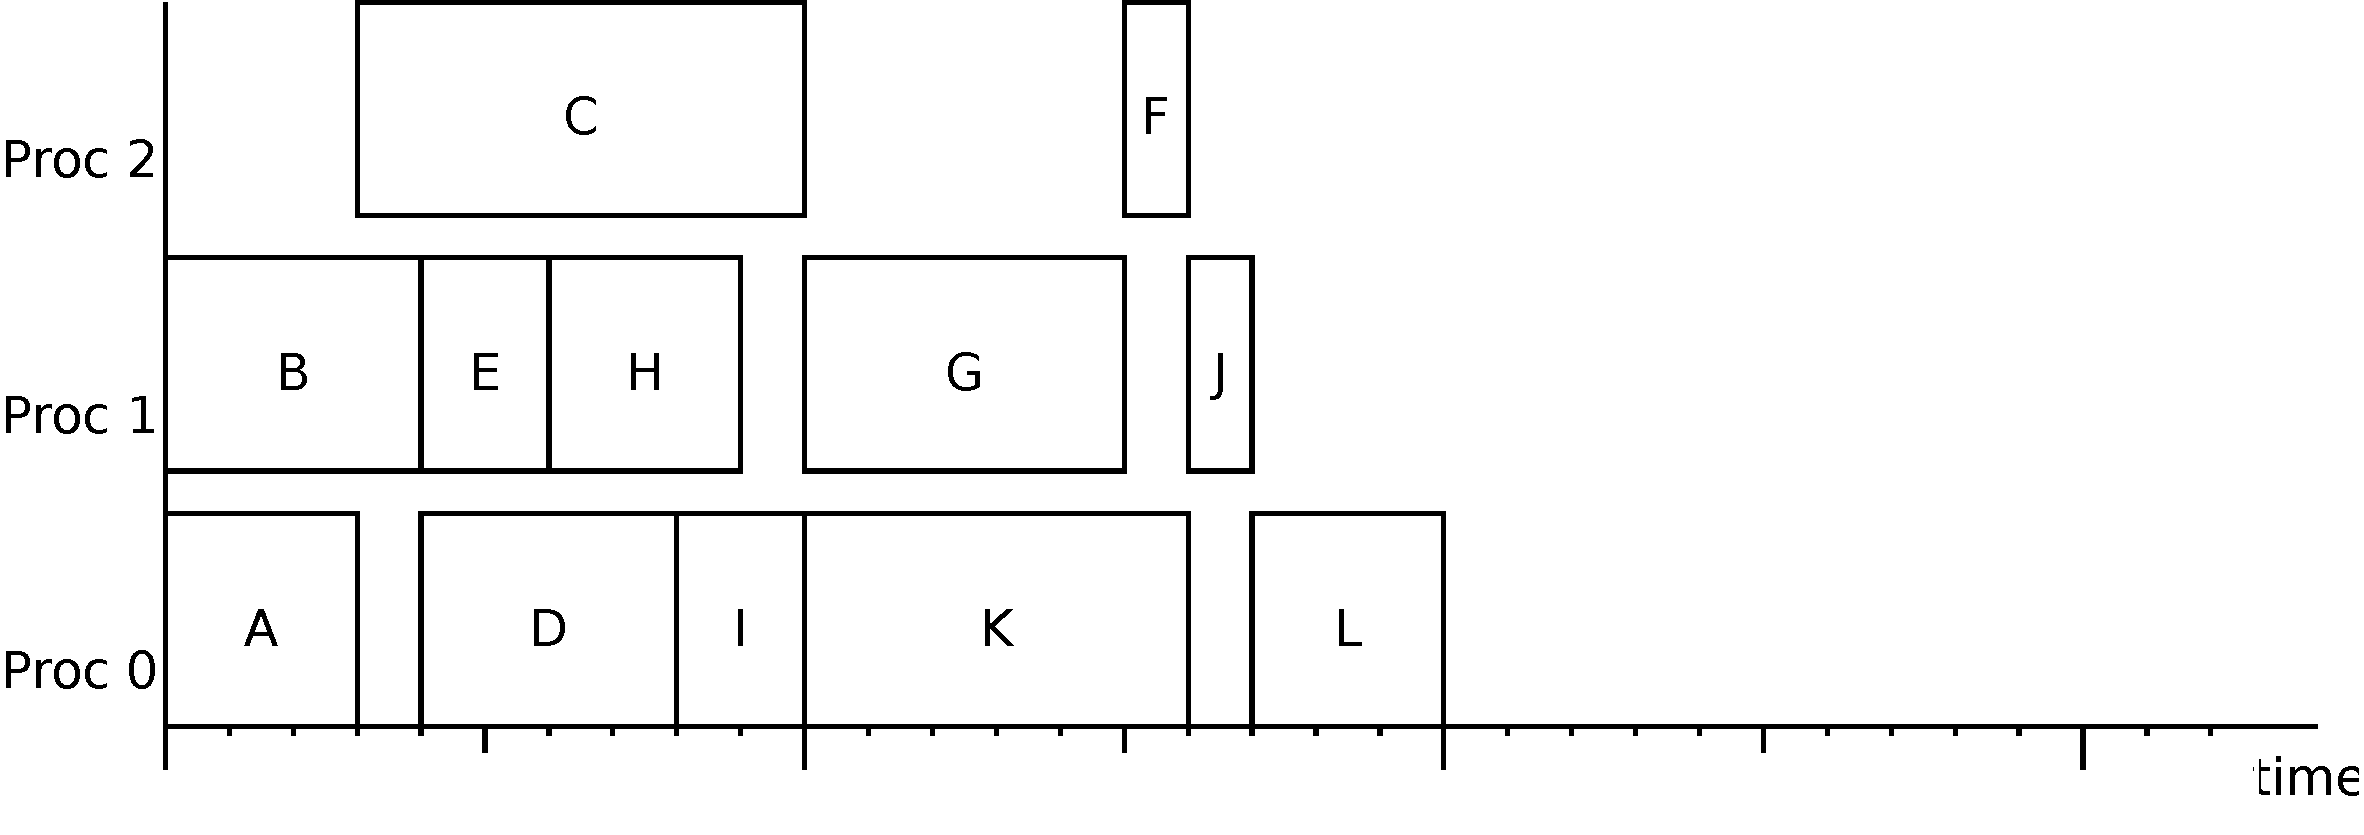
\includegraphics[width=.4\linewidth]{viz_figs/gantt-ls.pdf}
\end{frame}

\section{Assignments}

\begin{frame}
  \frametitle{Assignment Repository}

  Structured in course and topics

  \url{http://bridgesuncc.github.io/newassignments.html}
  

\end{frame}



\end{document}
%
